\setchapterpreamble[u]{\margintoc}
\chapter{Joint generation of multispectral and thermal point clouds}
\labch{multispectral_pc}
\label{sec:multispectral_pc}

\section*{About this chapter}

This chapter explains an efficient solution for the fusion of 1) visible, 2) thermographic and 3) multispectral information acquired by UAVs. Accordingly, we make effective the methodology proposed for image fusion in previous work \cite{lopez_framework_2021}, while also being extended to 3D. Furthermore, the proposed work is developed using massively parallel algorithms, supported by GPUs and multi-core CPUs. Commercial software is used as a baseline for evaluating the efficiency of our framework. Besides parallel processing, our approach is also focused on maximizing the size of point clouds. To this end, images with lower resolution are not directly processed to reconstruct 3D point clouds. Instead, the fusion methodology allows projecting additional sources of information over models derived from RGB estimations, which are known to generate results of higher dimensionality. 

Hence, the main contributions presented in this chapter are 1) the fusion of multiple imagery datasets from UAVs and 2) the generation of larger point clouds than current commercial software with 3) lower response time. The accurate colour aggregation in 3D points is ensured by taking into account the occlusion of foreground surfaces. Accordingly, the proposed solution reconstructs much more dense point clouds than notable commercial software (286\% on average), e.g., Pix4Dmapper and Agisoft Metashape, in much less time (-70\% on average). 

\section{On the generation of point clouds from multiple image sources}

Remote Sensing (RS) research concerns multiple acquisition devices and multispectral data obtained in different wavelength ranges. These are frequently visible, infrared and multispectral imagery, either collapsed into a few or hundreds of bands (hyperspectral). Thus, the main challenge of multiple sensing systems is to fuse all this information into a sole data model with multiple layers. Fusion methodologies have been long investigated to build multi-layer models that allow subsequent analyses to focus only on the data. From these models, Machine Learning \cite{padua_vineyard_2022} and Deep Learning \cite{jia_survey_2021, hu_hyperspectral_2022} represent a widespread field to extract further information. 

Among other factors, the raising interest in 3D models is possible due to the use of Unmanned Aerial Vehicles (UAV) in RS. In contrast to satellite imagery, UAVs provide a cost-efficient solution with higher spatial and temporal resolution \cite{singh_bibliometric_2022}. Nevertheless, cost-efficient vehicles and devices also lead to images with more defects and errors, either motivated by UAV instability \cite{akhoundi_khezrabad_new_2022} or the optical mechanism \cite{mohamad_screening_2021, lopez_framework_2021}. Besides this, the reduced flight altitude requires wider-angle lenses, thus generating more geometric distortions. Though some of these errors can be corrected, the number of steps for data fusion increases and so does the overall complexity. 

Finally, highly detailed 3D point clouds with hundreds of millions of points are complex to operate on commodity hardware. Despite this, they are required to provide in-depth analyses and valuable renderings \cite{schutz_rendering_2021}. As a result, the reconstruction and processing of large point clouds are computationally demanding tasks that require massively parallel algorithms and modern Graphics Processing Units (GPU) with increased capacity to operate many parallel threads. Therefore, solutions for fusing RS data are not solely aimed at providing accurate results, but also at efficiently generating them. The baseline for the reconstruction of 3D point clouds can be established using commercial software, with most of them taking advantage of GPUs to speed up the reconstruction \cite{jiang_efficient_2020}. Hence, their processing time is related both to the degree of parallelism as well as the size of input data. Accordingly, large point clouds are expected to worsen the performance, though they provide valuable data for mesh-like renderings and neighbourhood-derived processing (e.g., normal estimation).   

%-------------------------------------------------------------------------
\section{Correction and fusion of image datasets}

Images acquired either by thermographic or multispectral devices followed distinct distortion models, as previously explained. RGB and multispectral imagery present fisheye distortion due to their lower focal length, though it is especially visible in multispectral images. Thermographic lenses present a much larger focal length, thus following a pincushion distortion. However, distortion correction can be parameterized by five coefficients (radial and tangential distortion coefficients: $k_1, k_2, p_1, p_2, k_3$) in both cases, along with the camera matrix, $K$. Hence, the correction of every dataset is performed regardless of the camera source. An exception to this is given by multispectral, which defines its own distortion model defined by four distortion coefficients arranged in a 4th-degree equation. Note that distortion coefficients are not frequently read from image metadata. Instead, the bundle adjustment phase of SfM is used to estimate these coefficients. 

According to the surveying devices, two different pipelines are here established. The first pairs visible images with thermographic data by determining the image's id and the corresponding co-acquired thermal image. Similarly to the described pipeline, multispectral images are linked to the source RGB image. However, the latter image-matching is performed hierarchically, with the GRE layer being the master one. Hence, properties of other layers are calculated according to this, including the matrices for fusing images. The result of this section is a composite matrix for every RGB image, either relating it to a thermal or multispectral image. These are not related to more than one data source as they cannot be considered to be triggered synchronously. At this point, point clouds can be fed with additional information since their projection matrix to the RGB image plane is known. 

%-------------------------------------------------------------------------
\section{Projection in 3D point clouds}

The following step is to project 3D points into their original data source. As occurs with photogrammetric pipelines, the RGB point cloud may be first generated as it represents the most accurate and dense 3D result. From that representation, it can be enhanced by including additional spectral information at every point. Otherwise, a low-density version of the RGB point cloud would be generated from another data source. Hence, this work reuses the starting RGB point cloud, whose viewpoints are calibrated during SfM. For each one, the projection matrix, P$_c$, allows projecting 3D points into individual RGB image planes. From these, the previously computed inverse homography matrices allow translating RGB coordinates into a different Cartesian coordinate system. Hence, resulting projections corresponding to 3D points may fall out of image boundaries, thus not augmenting their information. As a result, augmented point clouds do not present the same dimensions as the first one, mainly in the boundaries. This is due to the smaller focal length of devices coupled to RGB, although they preserve the resolution (points per \si{\meter\squared}).

%-------------------------------------------------------------------------
\section{Occlusion}

The main drawback of the previously described projection is that spectral data from images could be projected into 3D points that were not visible from a flight viewpoint. Hence, this could lead to point clouds with incorrect colouring for additional layers. In this chapter, occlusion is solely handled using images that depict the scene depth as grayscale values, also known as \textit{z}-buffers. Due to the aim of this work, \textit{z}-buffers also store the index of the nearest point projected at each pixel. Otherwise, points projected at a pixel with higher depth are discarded.  From a $\infty$-filled image, points close to the viewpoint are projected to determine the minimum depth at each pixel, thus generating a \textit{z}-buffer similar to the output of depth sensors. However, \textit{z}-buffers with low resolution also lead to point clouds of lower density, as those generated by commercial software. To avoid this, the dimensionality of \textit{z}-buffers is upscaled by a factor $s$ to be determined in order to balance memory usage and the point cloud's density.

This task was solved using two different approaches. First, it was solved using OpenGL's built-in \textit{z}-buffers, and then, these were constructed from scratch using OpenGL's compute shaders.

\newcommand{\Points}{\textrm{P}\textsubscript{GPU}}
\newcommand{\Viewpoints}{\textrm{V}\textsubscript{CPU}}
\newcommand{\Space}{\hspace{1mm}}
\newcommand{\Zbuffer}{z\textrm{-buffer}\textsubscript{GPU}}
\newcommand{\ZbufferCPU}{z\textrm{-buffer}\textsubscript{CPU}}
\newcommand{\Indices}{\textrm{indices}\textsubscript{GPU}}
\newcommand{\Codes}{\textrm{codes}\textsubscript{GPU}}
\newcommand{\PCCardinality}{|\Points|}
\newcommand{\LeftPoints}{\textrm{n}_\textsubscript{left}}
\newcommand{\CurrentPoints}{\textrm{n}_\textsubscript{current}}
\newcommand{\MaxPoints}{\textrm{n}_\textsubscript{max}}
\newcommand{\NumGroups}{\textrm{n}_\textsubscript{groups}}
\newcommand{\Pointa}{\textrm{p}\textsubscript{3D}}
\newcommand{\Pointb}{\textrm{p}\textsubscript{2D}}

\subsection{OpenGL's rendering}

\begin{marginfigure}[.cm]
    \caption{OpenGL stages involved in drawing a point cloud.}
    \label{fig:occlusion_opengl_zbuffer_core}
    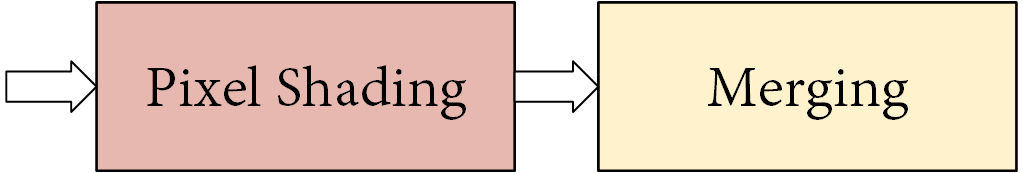
\includegraphics[width=\linewidth]{figs/multi_thermal_projection/occlusion_opengl_core.png}
\end{marginfigure}
Constructing \textit{z}-buffers is straightforwardly solved with OpenGL as it already addresses the occlusion in the rendering pipeline for point clouds (\verb|GL_POINTS|) and polygonal meshes. More specifically, it is the merging phase at the end of the traditional rasterization pipeline that is in charge of determining which primitive is visible at each pixel \cite{akenine-moller_real-time_2018}. However, the desired outcome of the visibility test is the buffer of indices belonging to those which are visible from a viewpoint. The workflow of this approach is shown in Figure \ref{fig:occlusion_opengl_zbuffer}.

\begin{marginfigure}[.2cm]
    \centering
    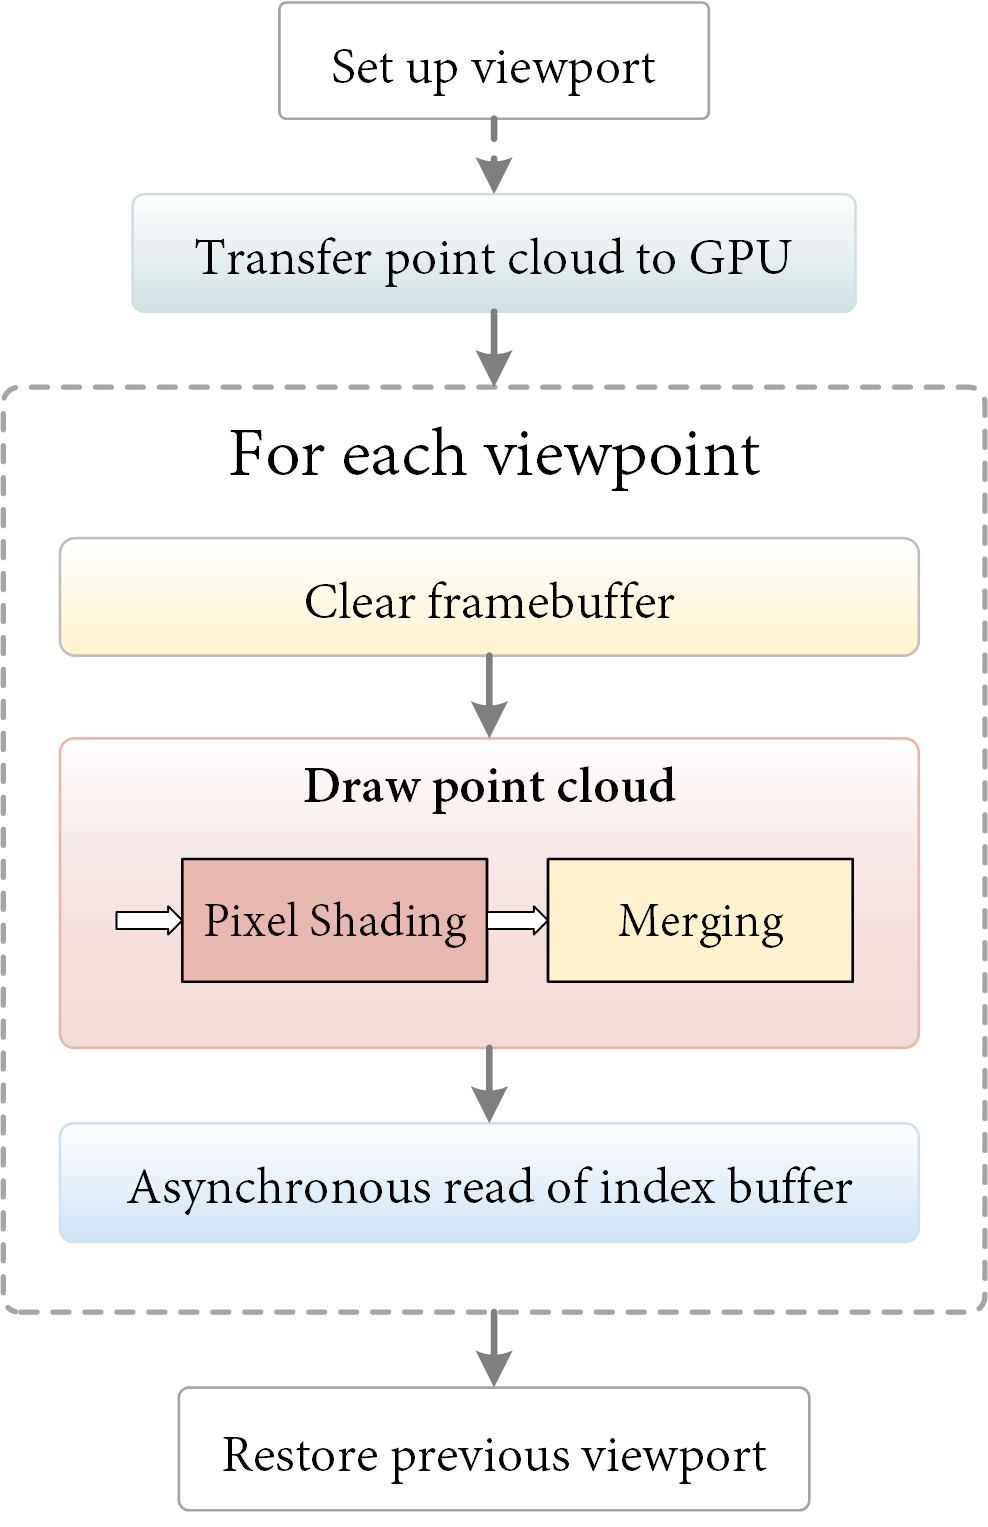
\includegraphics[width=\linewidth]{figs/multi_thermal_projection/occlusion_opengl.png}
    \caption{Workflow of the rendering-based methodology for a single batch of 3D points.}
    \label{fig:occlusion_opengl_zbuffer}
\end{marginfigure}
Points are transferred to the GPU as \verb|vec4| values (i.e., four floating-point numbers) to fit the data alignment rules of subsequent chapters. Also, a framebuffer comprising two textures of the same size is required; the first one collects point indices, whereas the second is a conventional \textit{z}-buffer. Restoring the framebuffer involves clearing the depth buffer and assigning a large value ($\infty$) to the indexing texture. Then, the whole point cloud is projected over the framebuffer, thus retrieving the nearest point visible at each pixel. Finally, the first texture is transferred to the CPU via asynchronous reading (\verb|glReadPixels|). In contrast to the limited GPU memory, CPU storage is large enough to store a buffer of size $\abs{V} \cdot x \cdot y$, provided that $V$ are images with a resolution of $x, y$.

However, large point clouds may not fit in a single GPU buffer. An alternative workflow is depicted in Figure \ref{fig:occlusion_opengl_zbuffer_multiple_batches}, with the maximum number of points depending on the storage capacity. However, the point cloud order is unknown and therefore iterations within this task are not disjoint. Consequently, the asynchronous reading involves reading the content of both depth and index buffers, which are then transferred to the GPU for the next batch of points, instead of being reset. Transferring the downloaded \textit{z}-buffer content to the GPU requires another rendering stage whose core is the built-in attribute \verb|gl_FragDepth| in the vertex shader. Also note that the framebuffer is not reset on each iteration, but only for the first batch of points. Another approach is to obtain the results for each viewpoint in a single iteration, though it implies a huge increase in data transfers from CPU to GPU. The latter requires transferring every point cloud batch once per viewpoint ($\abs{V} \cdot n_{b}$), instead of $n_{b}$, with $n_{b}$ being the number of point cloud subdivisions.

\begin{figure}[htb]
    \centering
    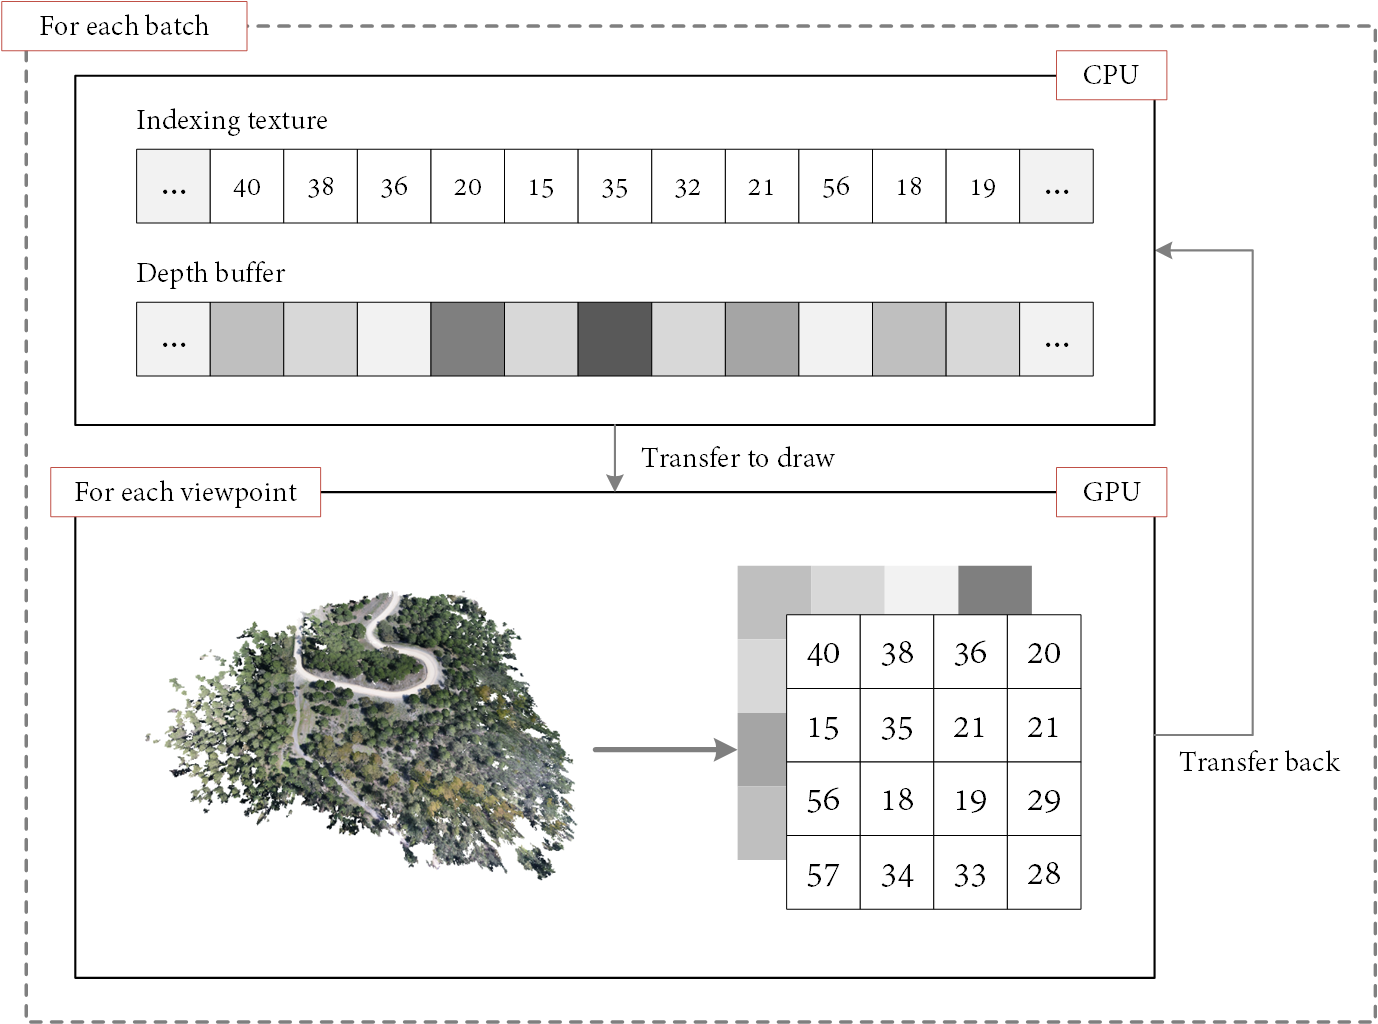
\includegraphics[width=\linewidth]{figs/multi_thermal_projection/multiple_batches_opengl_gpu.png}
    \caption{Overview of the rendering-based algorithm for multiple point cloud subdivisions.}
    \label{fig:occlusion_opengl_zbuffer_multiple_batches}
\end{figure}

\subsection{Compute shaders}

Compute shaders are general-purpose shaders for GPGPU programming, and therefore, they can be applied to tasks not related to rendering. Unlike OpenGL's rendering pipeline, \textit{z}-buffers are not provided in this shader stage and thus must be implemented as a low-level mechanism supported by buffers known as Shader Storage Buffer Objects (SSBO). Despite the lack of integrated \textit{z}-buffers, compute shaders provide a more efficient and flexible solution to read, write and perform trivial operations in buffers. Furthermore, it avoids some unnecessary stages from the rendering pipeline, including polygon rasterization and interpolations. 

\begin{algorithm}
  \begin{algorithmic}[1]
    \State Points are notated as \Points and $\Viewpoints$ are camera viewpoints whose images have dimensionality $x \cdot y$. The term id refers to \textrm{thread}\textsubscript{id} in the GPU. %\;
    \State Build $\Zbuffer \gets \textrm{uint64}(x \cdot y)$ and $\Indices \gets \textrm{uint}(x \cdot y)$ %\;
    \If{Sort \Points}
        \State $\Points \gets \textrm{sortPoints}(\Points)$   \Comment(Algorithm \ref{alg:sorting}) %\;
    \EndIf
    \Procedure{Build \textit{z}-buffers}{}
        \For {$v \Space \textrm{in} \Space \Viewpoints$}
            \State $M \gets v\textsubscript{projection}$ %\;
            \Procedure{Reset \textit{z}-buffer in GPU}{}
                \State $\Zbuffer_{i} \gets \textrm{UINT64\textsubscript{MAX}} \Space \forall i \in \left[0, x \cdot y\right[$ %\;
            \EndProcedure
            \Procedure{Fill \textit{z}-buffer in GPU}{$M$, $v_p$}
                \State $\Pointa \gets \Points\left[\textrm{id}\right]$ %\;
                \State $\Pointa \gets \left[M \cdot \left[\Pointa_x, \Pointa_y, \Pointa_z, 1\right]^T\right]_{xyz}^T$ %\;
                \State $\Pointb \gets \left[\Pointa_x / \Pointa_z, \Pointa_y / \Pointa_z\right]^T$ %\;
                \If{\Pointb \Space inside image}
                    \State $\textrm{dist} \gets \textrm{floatBitsToUint}(\textrm{length}(\Pointa - v_p))$ %\;
                    \State $\textrm{tag} \gets \textrm{p}\textsubscript{index} | \left(\textrm{dist} << 32\right)$ %\;
                    \State $\textrm{atomicMin}(\Zbuffer\left[\textrm{id}\right], \textrm{tag})$ %\;
                \EndIf
            \EndProcedure
            \Procedure{Obtain indices from \textit{z}-buffer}{}
                \State $\textrm{index}\left[\textrm{id}\right] \gets \Zbuffer\left[\textrm{id}\right] \& \textrm{UINT\textsubscript{MAX}}$ %\;
            \EndProcedure
            \State $\textrm{visible} \gets \Indices$ %\;
            \State Process $\textrm{visible}$ to assign point cloud colours %\;
        \EndFor
    \EndProcedure
    \caption{Simplest case for projecting points in \textit{z}-buffers, where all the points fit in the GPU's VRAM.}
    \label{alg:gpu_single_batch}
  \end{algorithmic}
\end{algorithm}

\begin{marginfigure}[.cm]
    \caption{Compute shader steps involved in drawing a point cloud.}
    \label{fig:occlusion_compute_shader_zbuffer_core}
    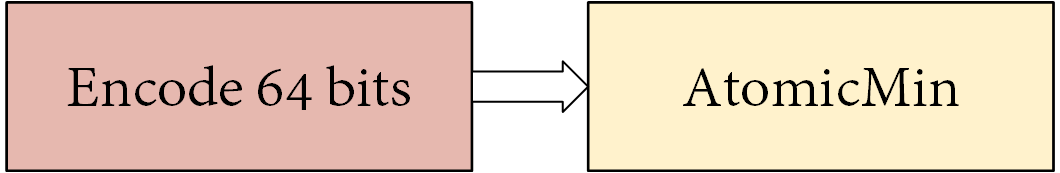
\includegraphics[width=\linewidth]{figs/multi_thermal_projection/occlusion_compute_shader_core.png}
\end{marginfigure}
Regarding memory allocation, \textit{z}-buffers are here modelled as integers of 64 bits (\verb|uint64_t|) using OpenGL's modern extensions, to be equally split between distance and index. Distance is not a numeric integer, $d \in \mathbb{R}$, though its low-level representation can be interpreted as an integer using \verb|floatBitsToUint|. For a viewpoint, $\textit{xyz}_c$, and a 3D point ($\textit{xyz}_p$) with index $i_p$, the Euclidean distance is computed, transformed into an integer and concatenated to $i_p$ (Equation \ref{eq:concatenation}). With this representation, fewer and greater comparisons work as usual. Thus, these operators can be applied to build a \textit{z}-buffer by selecting the minimum distance while also carrying the point index. To this end, the atomic \textit{min.} operator (\verb|atomicMin|) is used.
\begin{equation}
\label{eq:concatenation}
z_{k, l} \gets d(\textit{xyz}_p, \textit{xyz}_c) ^\frown x_p
\end{equation}

The procedure to project the point cloud into $z$-buffers is following described in Algorithm \ref{alg:gpu_single_batch} if it fits in the GPU's VRAM and the maximum size OpenGL's buffers (see Figure \ref{fig:occlusion_compute_shader_zbuffer}). Otherwise, Algorithm \ref{alg:gpu_multiple_batch} is followed. Note that the second scenario omits the smaller procedures shown in Algorithm \ref{alg:gpu_single_batch}. Because data transfers of $z$-buffers in CPU $\leftrightarrow$ GPU are notably smaller, point batches are iterated in the outer $\textit{for}$ and thus only transferred once. Instead, each viewpoint's $z$-buffer is transferred once per point batch. Once all the points have been projected into every $z$-buffer, the indices indicating which points are visible are obtained, as proposed in Algorithm \ref{alg:gpu_single_batch}.
\begin{marginfigure}[.3cm]
    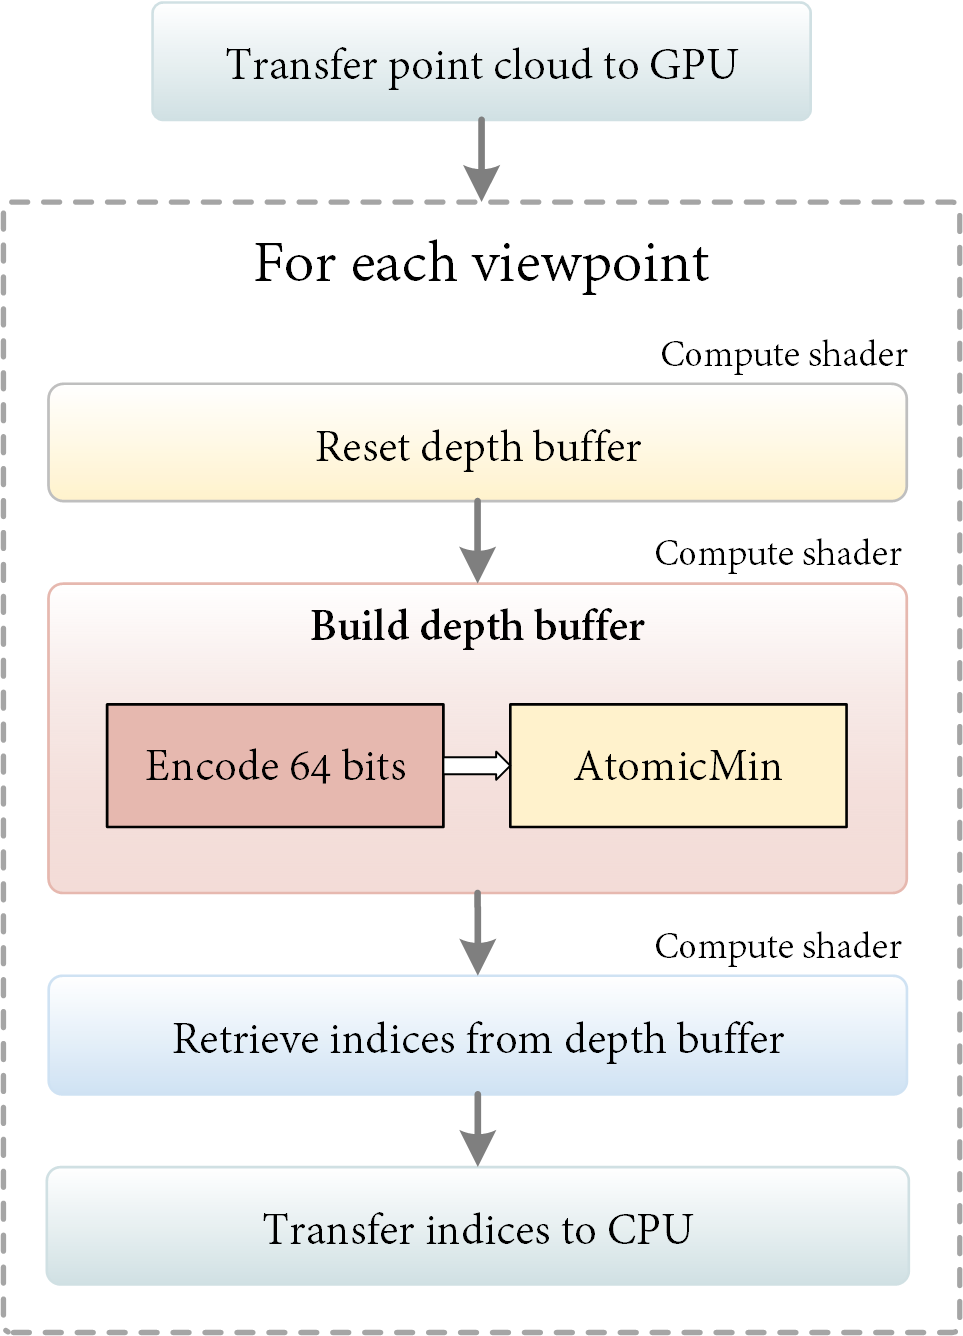
\includegraphics[width=\linewidth]{figs/multi_thermal_projection/occlusion_compute_shader.png}
    \caption{Overview of compute shader methodology for a single batch of 3D points.}
    \label{fig:occlusion_compute_shader_zbuffer}
\end{marginfigure}

\begin{algorithm}
  \begin{algorithmic}[1]
    \State $\Points$ refers to points, $\Viewpoints$ are camera viewpoints whose images have dimensionality $x \cdot y$ and $\MaxPoints$ is the maximum number of points that can be allocated in the GPU. %\;
    \State Build $\ZbufferCPU \gets \textrm{uint64}(x \cdot y \cdot |\Viewpoints|)$ %\;
    \State $\ZbufferCPU_{i} \gets \textrm{UINT64\textsubscript{MAX}} \Space \forall i \in \left[0, x \cdot y \cdot |\Viewpoints|\right[$ %\;
    \State Build $\Zbuffer \gets \textrm{uint64}(x \cdot y)$ and $\Indices \gets \textrm{uint}(x \cdot y)$ %\;
    \State $\LeftPoints \gets \PCCardinality$ %\;
    \If{Sort \Points}
        \State $\Points \gets \textrm{sortPoints}(\Points)$   \Comment(Algorithm \ref{alg:sorting}) %\;
    \EndIf
    \While{$\LeftPoints > 0$}
        \State $\CurrentPoints \gets \textrm{min}(\LeftPoints, \MaxPoints)$ %\;
        \State Transfer point batch to GPU %\;
        \For {$v \Space \textrm{in} \Space \Viewpoints$}
            \State Transfer to GPU part of $\ZbufferCPU$ from $v$ %\;
            \State Complete $\Zbuffer$ with current point batch %\;
            \State Read $\Zbuffer$ into the pointer of $\ZbufferCPU$ %\;
        \EndFor
        \State Update $\LeftPoints$ %\;
    \EndWhile
    \For {$v \Space \textrm{in} \Space \Viewpoints$}
        \State Transfer to GPU part of $\ZbufferCPU$ from $v$ %\;
        \State Split indices from \Zbuffer into \Indices %\;
        \State $\textrm{visible} \gets \Indices$ %\;
        \State Process $\textrm{visible}$ to assign point cloud colours %\;
    \EndFor
    \caption{The point vector is split if it does not fit in the GPU's VRAM during their projection in \textit{z}-buffers.}
    \label{alg:gpu_multiple_batch}
  \end{algorithmic}
\end{algorithm}

\subsection{CUDA}

The CUDA kernel for computing the nearest 3D point for every pixel and viewpoint is analogous to the compute shader workflow. The main challenge in the CUDA implementation is to overlap the CPU $\leftrightarrow$ GPU transfers with the GPU processing as much as possible. The use of multiple CUDA streams exploits asynchronous transfer operations and kernel executions to achieve an efficient result. Hence, points from a batch are projected in the CUDA kernel meanwhile the next batch is being transferred to GPU. Similarly, results are downloaded from the CPU while a viewpoint is being processed by the current kernel.

\lstinputlisting[language=c++, caption={Overlapping execution of different data streams per point cloud batch.}, label=code:occlusionCUDA]{code/cuda_occlusion.cpp}

%-------------------------------------------------------------------------
\section{Point cloud sorting}

\begin{marginfigure}[1cm]
    \centering
    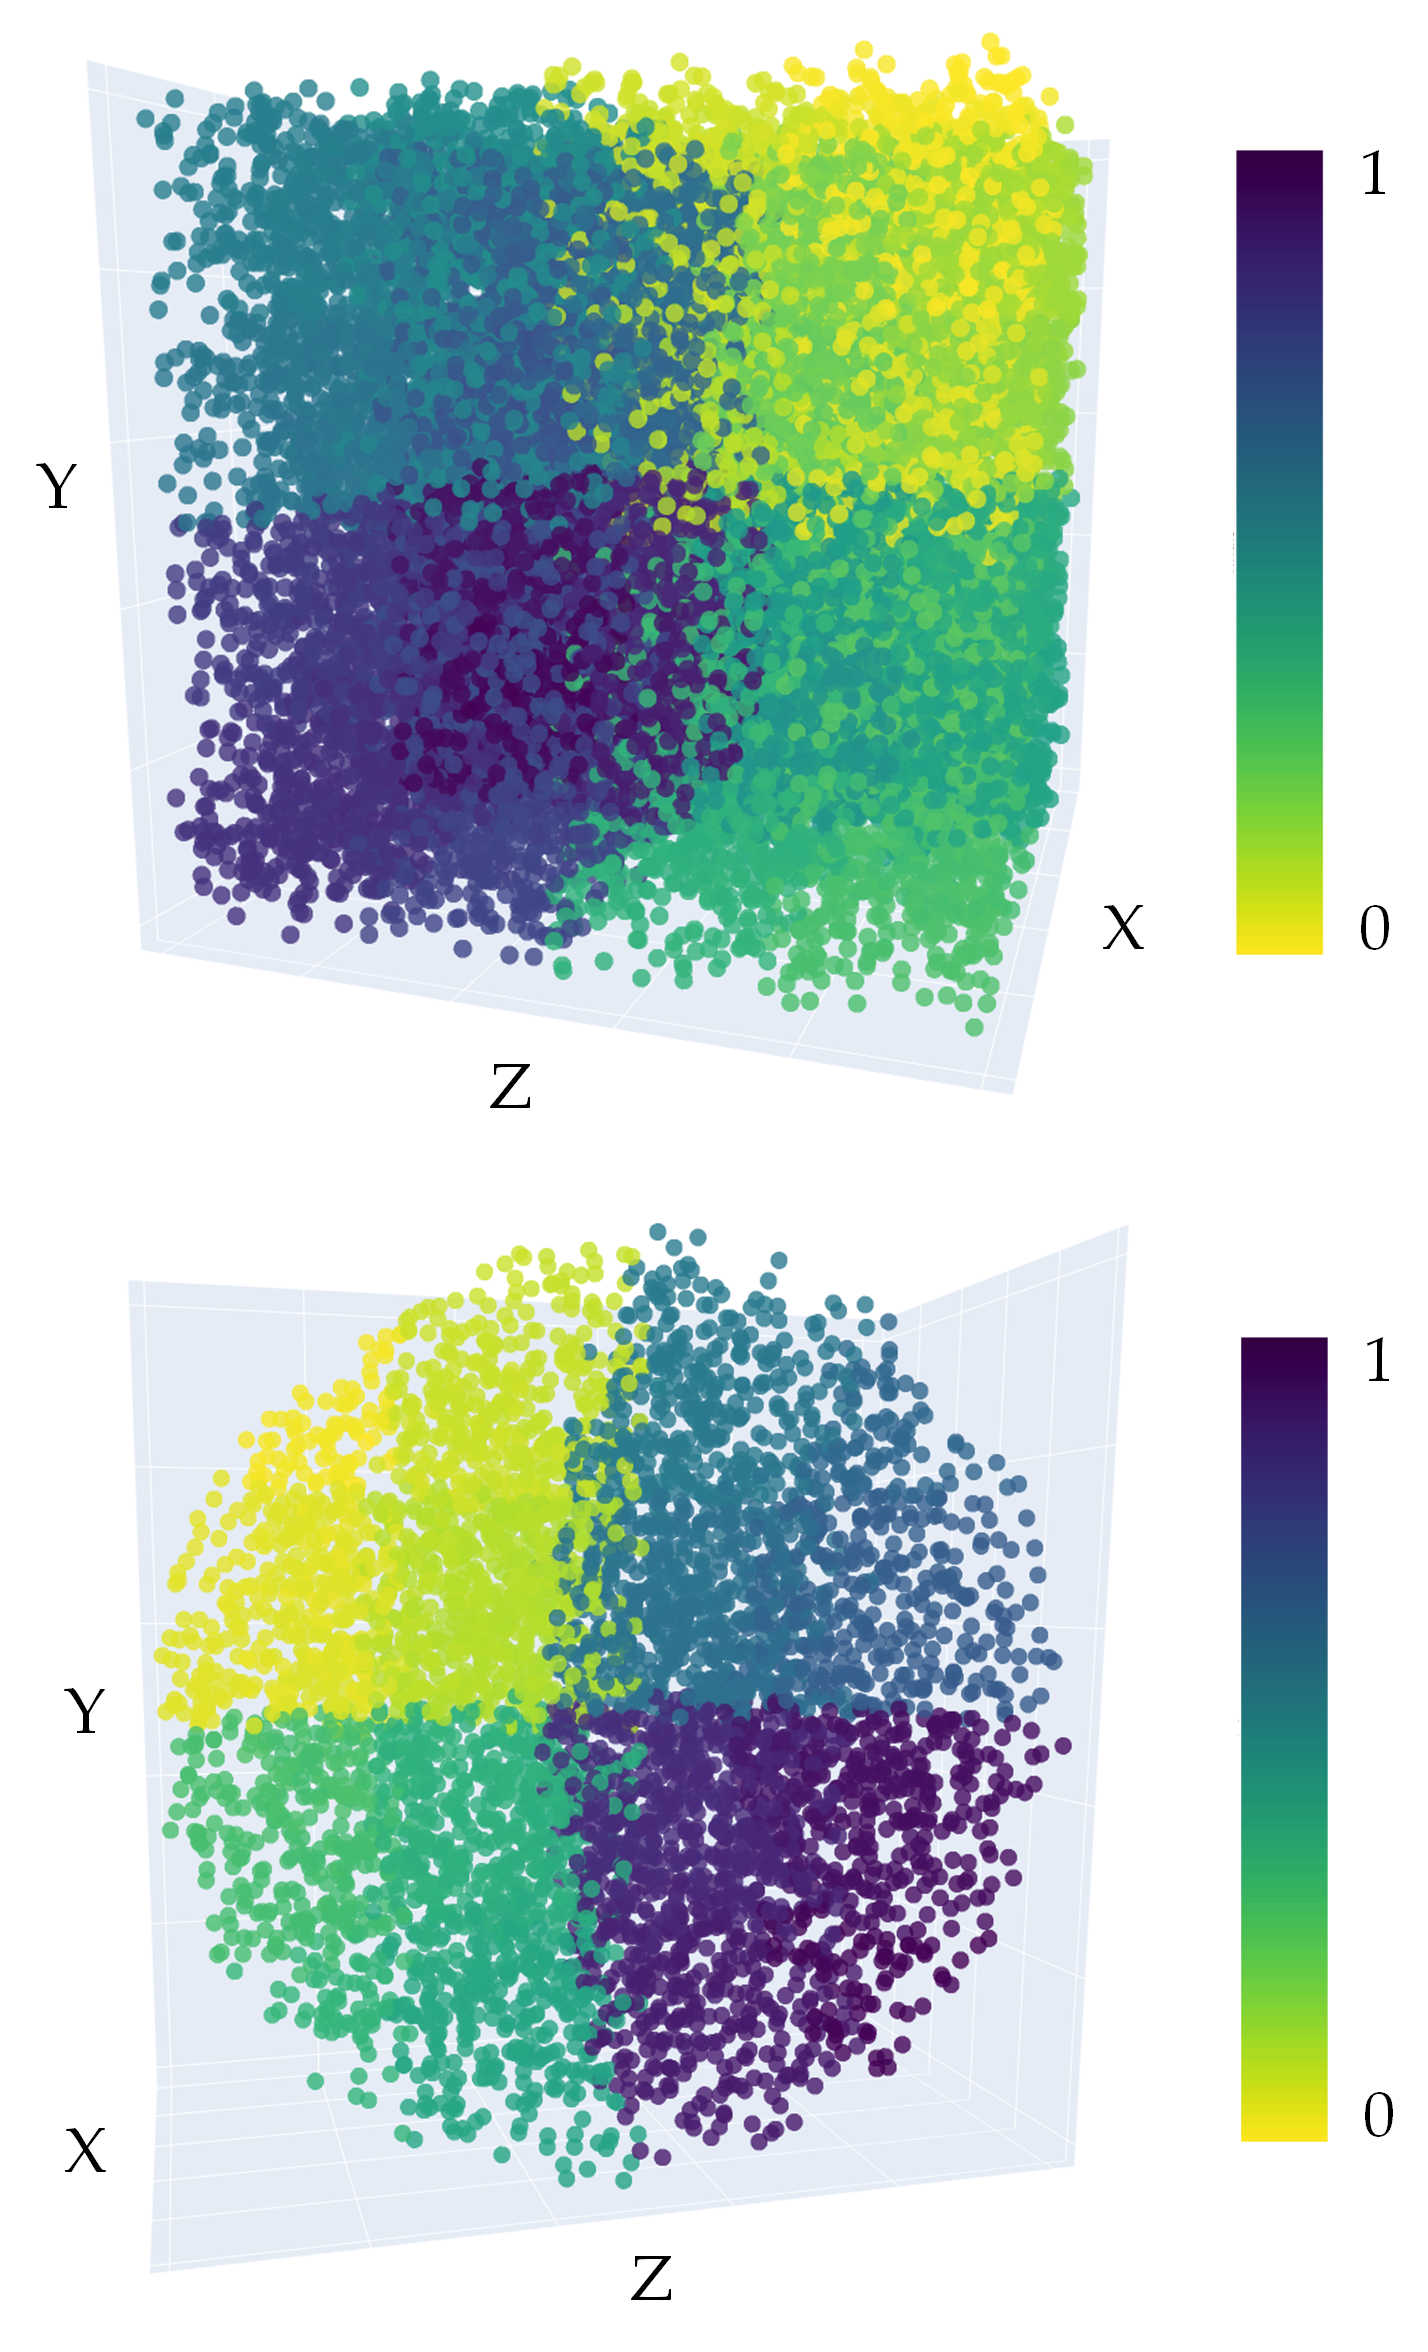
\includegraphics[width=\linewidth]{figs/multi_thermal_projection/point_cloud_morton.png}
    \caption{Colouring of two randomized point clouds in [0, 1] according to Morton encoding with 30 bits. }
	\label{fig:morton_point_cloud}
\end{marginfigure}
Point clouds generated by software present an unknown order regardless of their coordinates, \textit{xyz}. However, the outcome of previous projections is highly influenced by the sampled 3D volume. As a result, points within an area could be visible from a camera viewpoint, whereas other parts of the point cloud may be discarded. Consequently, point clouds of unknown order also require unordered updates in memory buffers. However, organized updates are known to be more efficient due to faster memory writing. Although there is no such ordering in 3D space, there exist methods for the hierarchical clustering of geometry, such as the \textit{Z}-order curve (also known as Morton curve, depicted in Figure \ref{fig:morton_point_cloud}). The outcome is a 1D buffer where close indices in memory are linked to spatially close 3D points. 

\begin{algorithm}
  \begin{algorithmic}[1]
    \State $\Points$ refers to the point cloud and $\MaxPoints$ is the maximum number of points that can be allocated in the GPU. %\;
    \State $\LeftPoints \gets \PCCardinality$ %\;
    \State $\textrm{indices} \gets \textrm{uint}\left[\PCCardinality\right]$ %\;
    \While{$\LeftPoints > 0$}
        \State $\CurrentPoints \gets \textrm{min}(\LeftPoints, \MaxPoints)$ %\;
        \State Transfer the following $\CurrentPoints$ batch to GPU %\;
        \Procedure{Sort in GPU}{}
            \State $\Codes \gets \textrm{mortonGPU}(\Points)$ %\;  
            \State $\textrm{indices} \gets \textrm{RadixSort}(\Points, \Codes)$ %\;
            \Procedure{$\textrm{RadixSort}(\Points, \Codes)$}{}
                \For {$\textrm{bit} \gets 0 \to 30$} 
                    \State Apply bit mask $1 << \textrm{bit to} \Points$ %\;
                    \State Up-sweep phase of prefix scan %\;
                    \State Reset last position to zero %\;
                    \State Down-sweep phase of prefix scan %\;
                    \State Reorder \Points with new positions %\;
                \EndFor
            \EndProcedure
        \EndProcedure
        \Procedure{Sort in multi-core CPU}{}
            \If{Shuffle}
                \State $\NumGroups \gets \lceil \CurrentPoints / \textrm{n}\textsubscript{shuffle} \rceil$ %\;
                \State rdn\textsubscript{group} $\gets \textrm{RandomVector}(\NumGroups, 0, 1)$ %\;
                \State iota\textsubscript{group} $\gets \bigl[0, 1, ..., \NumGroups-1 \bigr]$ %\;
                \State id\textsubscript{old}, id\textsubscript{new} $\gets$ Sort($\textrm{rdn\textsubscript{group}}, \textrm{iota}\textsubscript{group}$) %\;
                \For {group in $\left(\textrm{id}\textsubscript{old}, \textrm{id}\textsubscript{new} \right)$}
                    \State Move point batch from $\textrm{id}\textsubscript{old}$ to $\textrm{id}\textsubscript{new}$ %\;
                \EndFor
            \Else
                \State Reorder points with indices %\;
            \EndIf
        \EndProcedure
        \State Update \Points \Space and $\LeftPoints$ with $\CurrentPoints$ %\;
    \EndWhile
    \caption{Point cloud sorting.}
    \label{alg:sorting}
  \end{algorithmic}
\end{algorithm}

For large point clouds, changing their order presents a significant delay even for the most efficient sorting algorithms. Therefore, GPGPU programming allows sorting them in parallel to reduce the response time during the projection procedure. In this work, Radix sort is used and adapted to GPU programming by splitting it into two different steps: 1) up-sweep (reduce) and 2) down-sweep \cite{nguyen_gpu_2007}. Following this approach, the buffer is sorted with a complexity of $\mathcal{O}(m\log{}n)$, with $m$ being the number of bits and $n$ being the number of points. Prior to sorting, \textit{xyz} coordinates are converted to values of 30 bits ($m$) that encodes individual coordinates (10 bits for each one). These have been previously revised as Morton codes, though they can have a variable bit length.

Despite the enhancement derived from sorting, GPU-based algorithms are handled on the GPU through work groups. These are small groups of threads that are allowed to share data. Thus, the main drawback of sorting the point cloud buffer as a whole is that the workload is not uniformly shared among work groups. Instead, the ordered buffer can be shuffled according to the size of the workgroups. The algorithmic flow for the described sort configuration is shown in Algorithm \ref{alg:sorting}. First, points are sorted with Radix Sort following the Morton encoding. Otherwise, a random order is used. Then, the point buffer can be reordered according to groups of size n\textsubscript{shuffle}. The second stage is implemented as a multi-core CPU algorithm rather than in the GPU to avoid duplicating large point buffers with limited VRAM.

\section{Alignment of heterogeneous data sources}

Image matching was performed in visible and alternative imagery from the same sensor. This way, images are known to be acquired with a similar timestamp, and thus ECC converges in a reasonable time. However, RGB point clouds can be reused for different data sources whether they are represented in the same local coordinate system. Despite georeferencing providing accurate positioning, point clouds from distinct data sources may not exactly overlap. Hence, point clouds are further processed by finding the rigid transformation matrix that is able to align both of them with a precision below a threshold (Figure \ref{fig:icp}). It is performed with the Iterative Closest Point (ICP) algorithm.

\begin{figure}[ht]
    \centering
    \includegraphics[width=\linewidth]{figs/multi_thermal_projection/ICP.png}
    \caption{ICP registration process: a) RGB point cloud from the first dual device, b) RGB point cloud from the second dual device, and c) both point clouds aligned by minimizing their distance, with $G$ referring to a Global system.}
    \label{fig:icp}
\end{figure}

\section{Experimental results and discussion}

\begin{figure*}
    \centering
    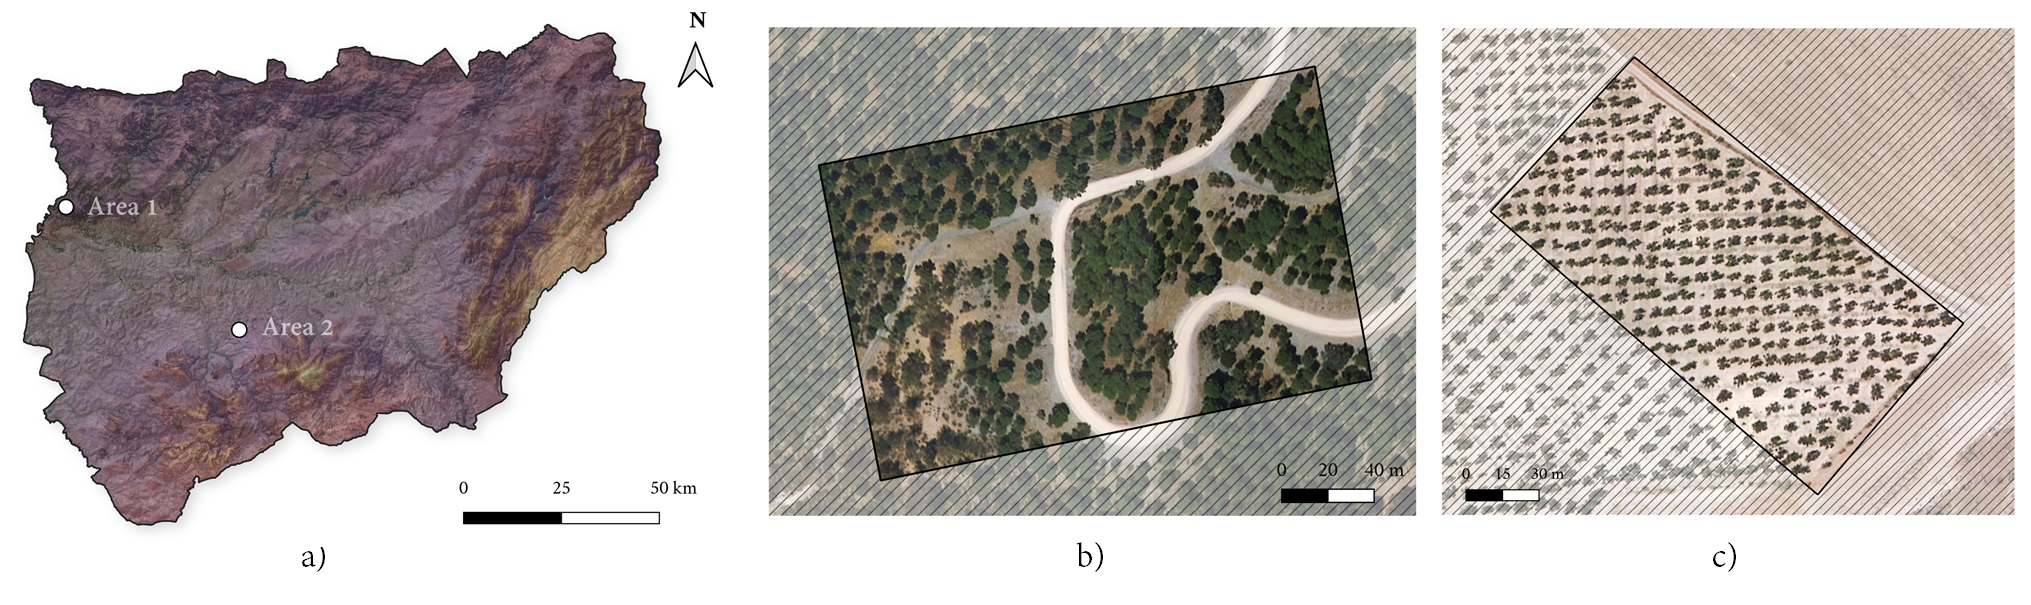
\includegraphics[width=\linewidth]{figs/multi_thermal_projection/study area.png}
    \caption{Overview of surveyed region and areas. a) Region of Jaén, b) forest and c) olive grove.   }
	\label{fig:occlusion_study_area}
\end{figure*}

In this section, the proposed methodology is compared with other notable software solutions for building multispectral and thermal point clouds, such as Pix4Dmapper or Agisoft Metashape, using their highest-quality reconstruction. The carried tests are focused on obtaining the response time and point cloud size, although some reconstructions from these solutions also present geometrical errors. The evaluation was performed on a PC with AMD Ryzen Threadripper 3970X 3.6 GHz, 256 GB RAM, two Nvidia RTX A6000 GPUs and Windows 10 OS. The proposed methodology was implemented in C++ using the Open Graphics Library (OpenGL) both for rendering and computing. Besides GPU computing, CPU-based methods were also accelerated using the OpenMP multithreading framework.

The RGB point clouds used as input for our method consist of 115M (multispectral) and 97M (thermal) points for the first dataset, whereas the second dataset yields point clouds with a dimensionality of 126M and 96M points. To further stress this evaluation and achieve higher point density, we have used a single depth buffer resolution, $d\gets 10$. Regarding point cloud order, points are initially shuffled to show the benefits of spatial sorting. Apart from this, two different setups are here shown: 1) sorted with Morton codes and 2) sorted and shuffled in small groups. The experimental results are obtained by repeating every test four times and averaging them. 

\begin{kaobox}[frametitle=OpenGL and CUDA comparison]
This chapter comprises the last of this dissertation, with compute shaders being the preferred solution. Other presented approaches use OpenGL's rendering pipeline as well as the CUDA framework to perform this very same operation. However, the latter comparison was performed in a work published in the \textbf{Proceedings of the 2021 Spanish Conference in Computer Graphics}. In this work, tests were performed on a PC with Intel Core i9-9900 3.1 GHz, 48 GB RAM, RTX 2080 Ti GPU with 11 GB RAM (Turing architecture) and Windows 10 OS, using C++, CUDA and OpenGL. The dataset was the first here explained (forestry area), although the input cloud had 271 million points was viewed from 1352 viewpoints. A simplified version of this consisted of 66 million points and 180 viewpoints. 
\end{kaobox}

Regarding the configuration of commercial solutions, the steps of image alignment and reconstruction of a dense point cloud (i.e., densification) were performed with the highest quality. Since both of them are known to be able to use CUDA-enabled GPUs, they were enabled to accelerate their pipeline on the GPU. Furthermore, the latter is known to be accelerated with the multi-GPU framework CUDA and therefore, was expected to perform better since two GPUs were available.  
\subsection{Study area}

The proposed method has been evaluated over two different environments located in the region of Jaén, Spain. To show its effectiveness in multiple fields, data depicting 1) a forestry area and 2) an olive grove was processed. Hence, the fusion of information works well in scenarios with more significant features (2) and not recognizable features (1). Figure \ref{fig:occlusion_study_area} shows the location of both areas. The flight altitude was 454\si{\meter} and 595\si{\meter}, respectively. The forestry scene is composed of repetitive patterns from vegetation and human-made structures. The first area covers nearly 1.97\si{\hectare}, whereas the second comprises 2.44\si{\hectare}.

\subsection{Image processing}

The image alignment stage is configured according to the ECC parameters: 1) the number of iterations to converge and 2) the aimed precision. The first is set to 400 iterations to sufficiently cover the number of required iterations. The precision is set to the default value, $\epsilon \gets 1^{-3}$. Besides these parameters, the dimensionality of the compared images is also relevant since the lesser number of details also implies a faster convergence. However, images were not downscaled in this study to guarantee the quality of the alignment. Finally, the hierarchical alignment of multispectral images is also studied by means of confusion matrices that show the correlation of pairs of bands. Accordingly, Figure \ref{fig:occlusion_confusion_matrices} justifies the hierarchy shown in Figure \ref{fig:ecc_hierarchy}. Note that NIR and REG layers are reciprocally the most similar. However, REG images are more similar to the root, GRE, and thus NIR layers were aligned to REG images.

\begin{figure*}[ht]
    \centering
    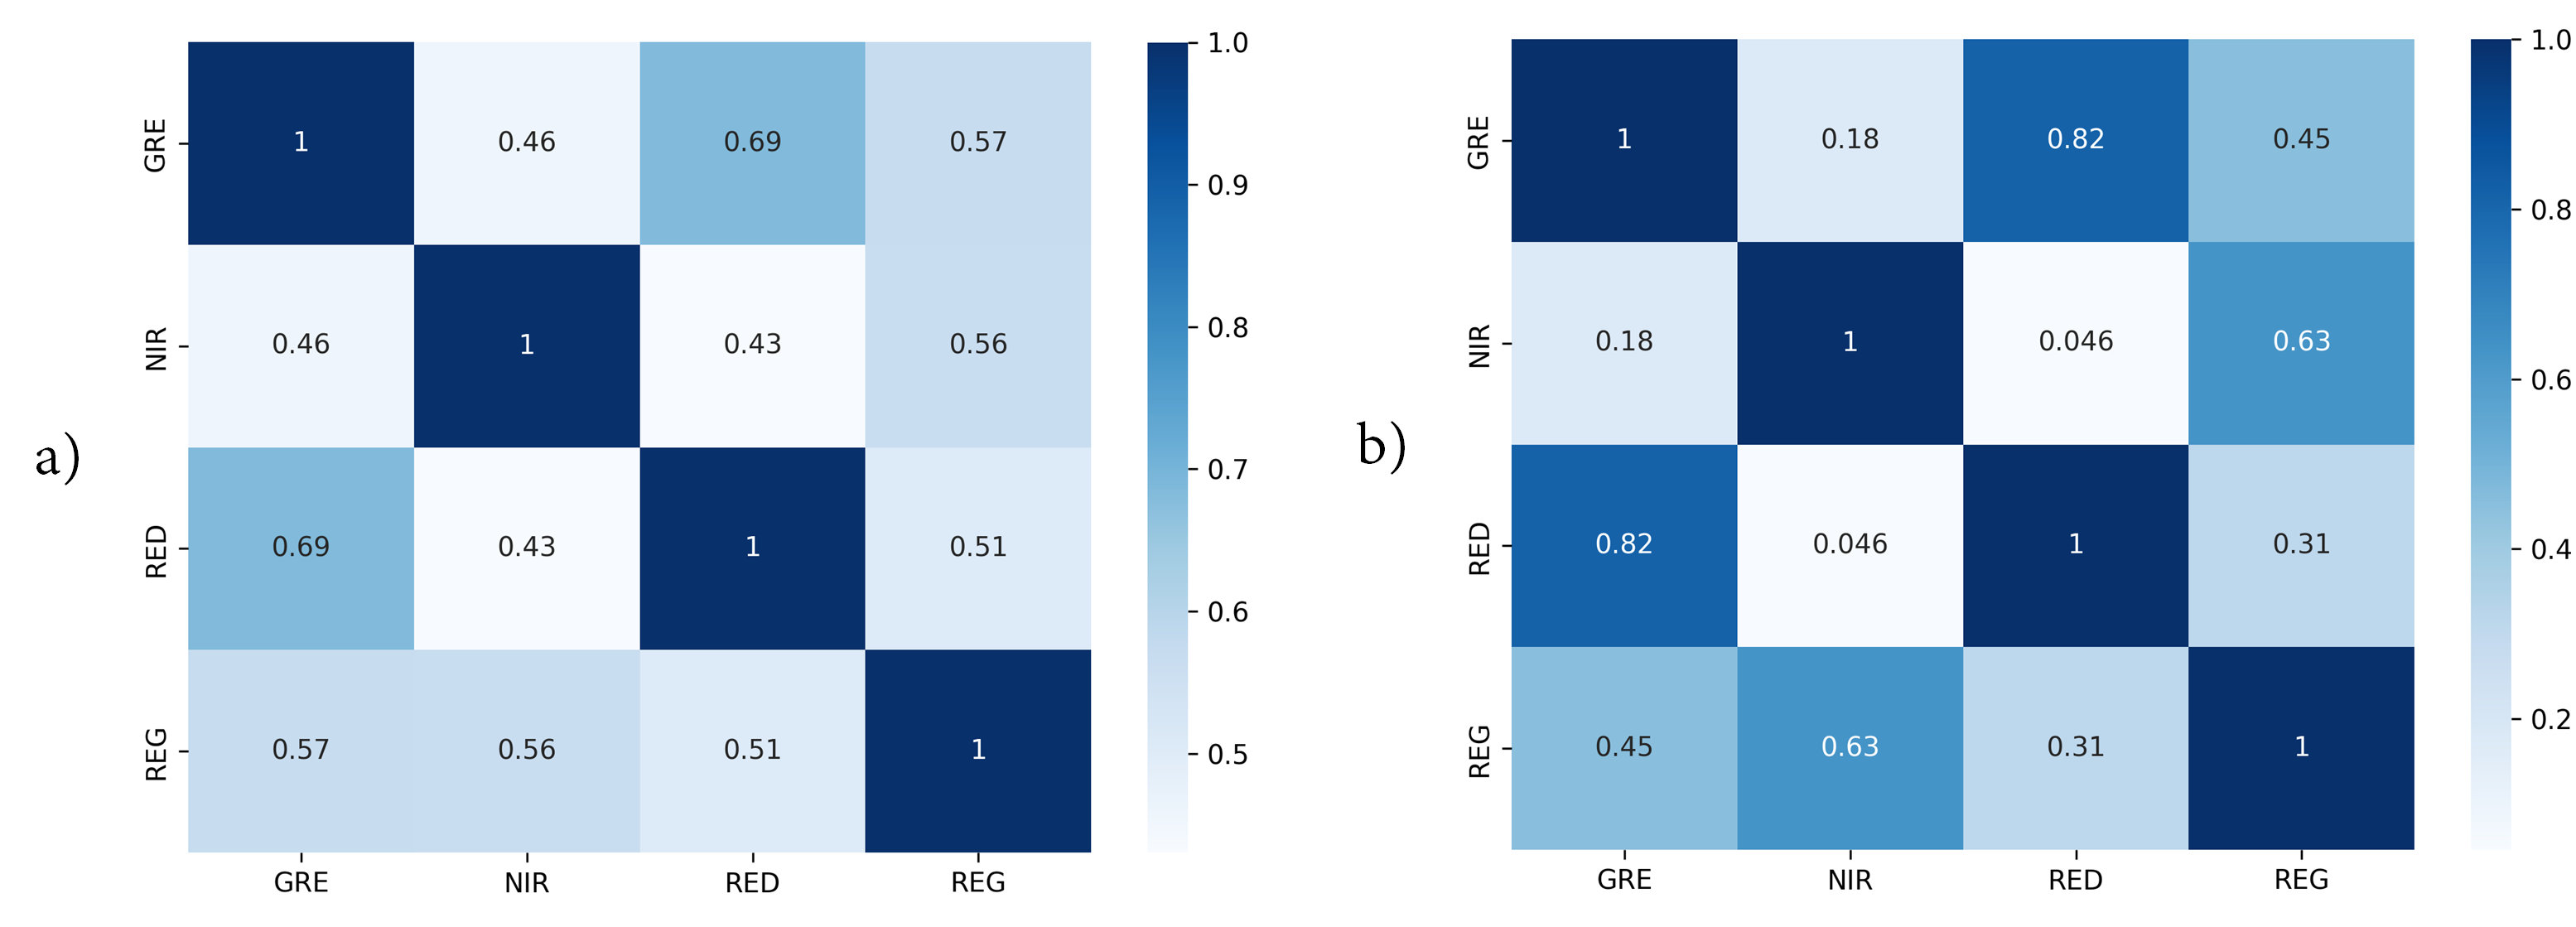
\includegraphics[width=.9\linewidth]{figs/multi_thermal_projection/results/confusion_matrices.png}
    \caption{Confusion matrix to depict the similarity of multispectral images in the first and second dataset (a) and b), respectively).}
    \label{fig:occlusion_confusion_matrices}
\end{figure*}

Regarding the sought precision, images were aligned using $\epsilon \gets 10^{-5}$ for all the data sources, according to the similarity observed in Figure \ref{fig:ecc_precision}. The similarity was here normalized to improve the readability of the chart, though the average intensity differences through the experimental results were observed to be in the order of $1^-3$. Lower values (higher exponent) harden the convergence of the ECC alignment while also increasing the latency in the order of \si{\milli\second}. Hence, an intermediate value that balances both intensity and response time was used. On the other hand, the number of iterations is set to guarantee the procedure converges before reaching such a number. Therefore, a large value such as $\textit{it} \gets 400$ was enough for our case studies.

\begin{figure}[ht]
    \centering
    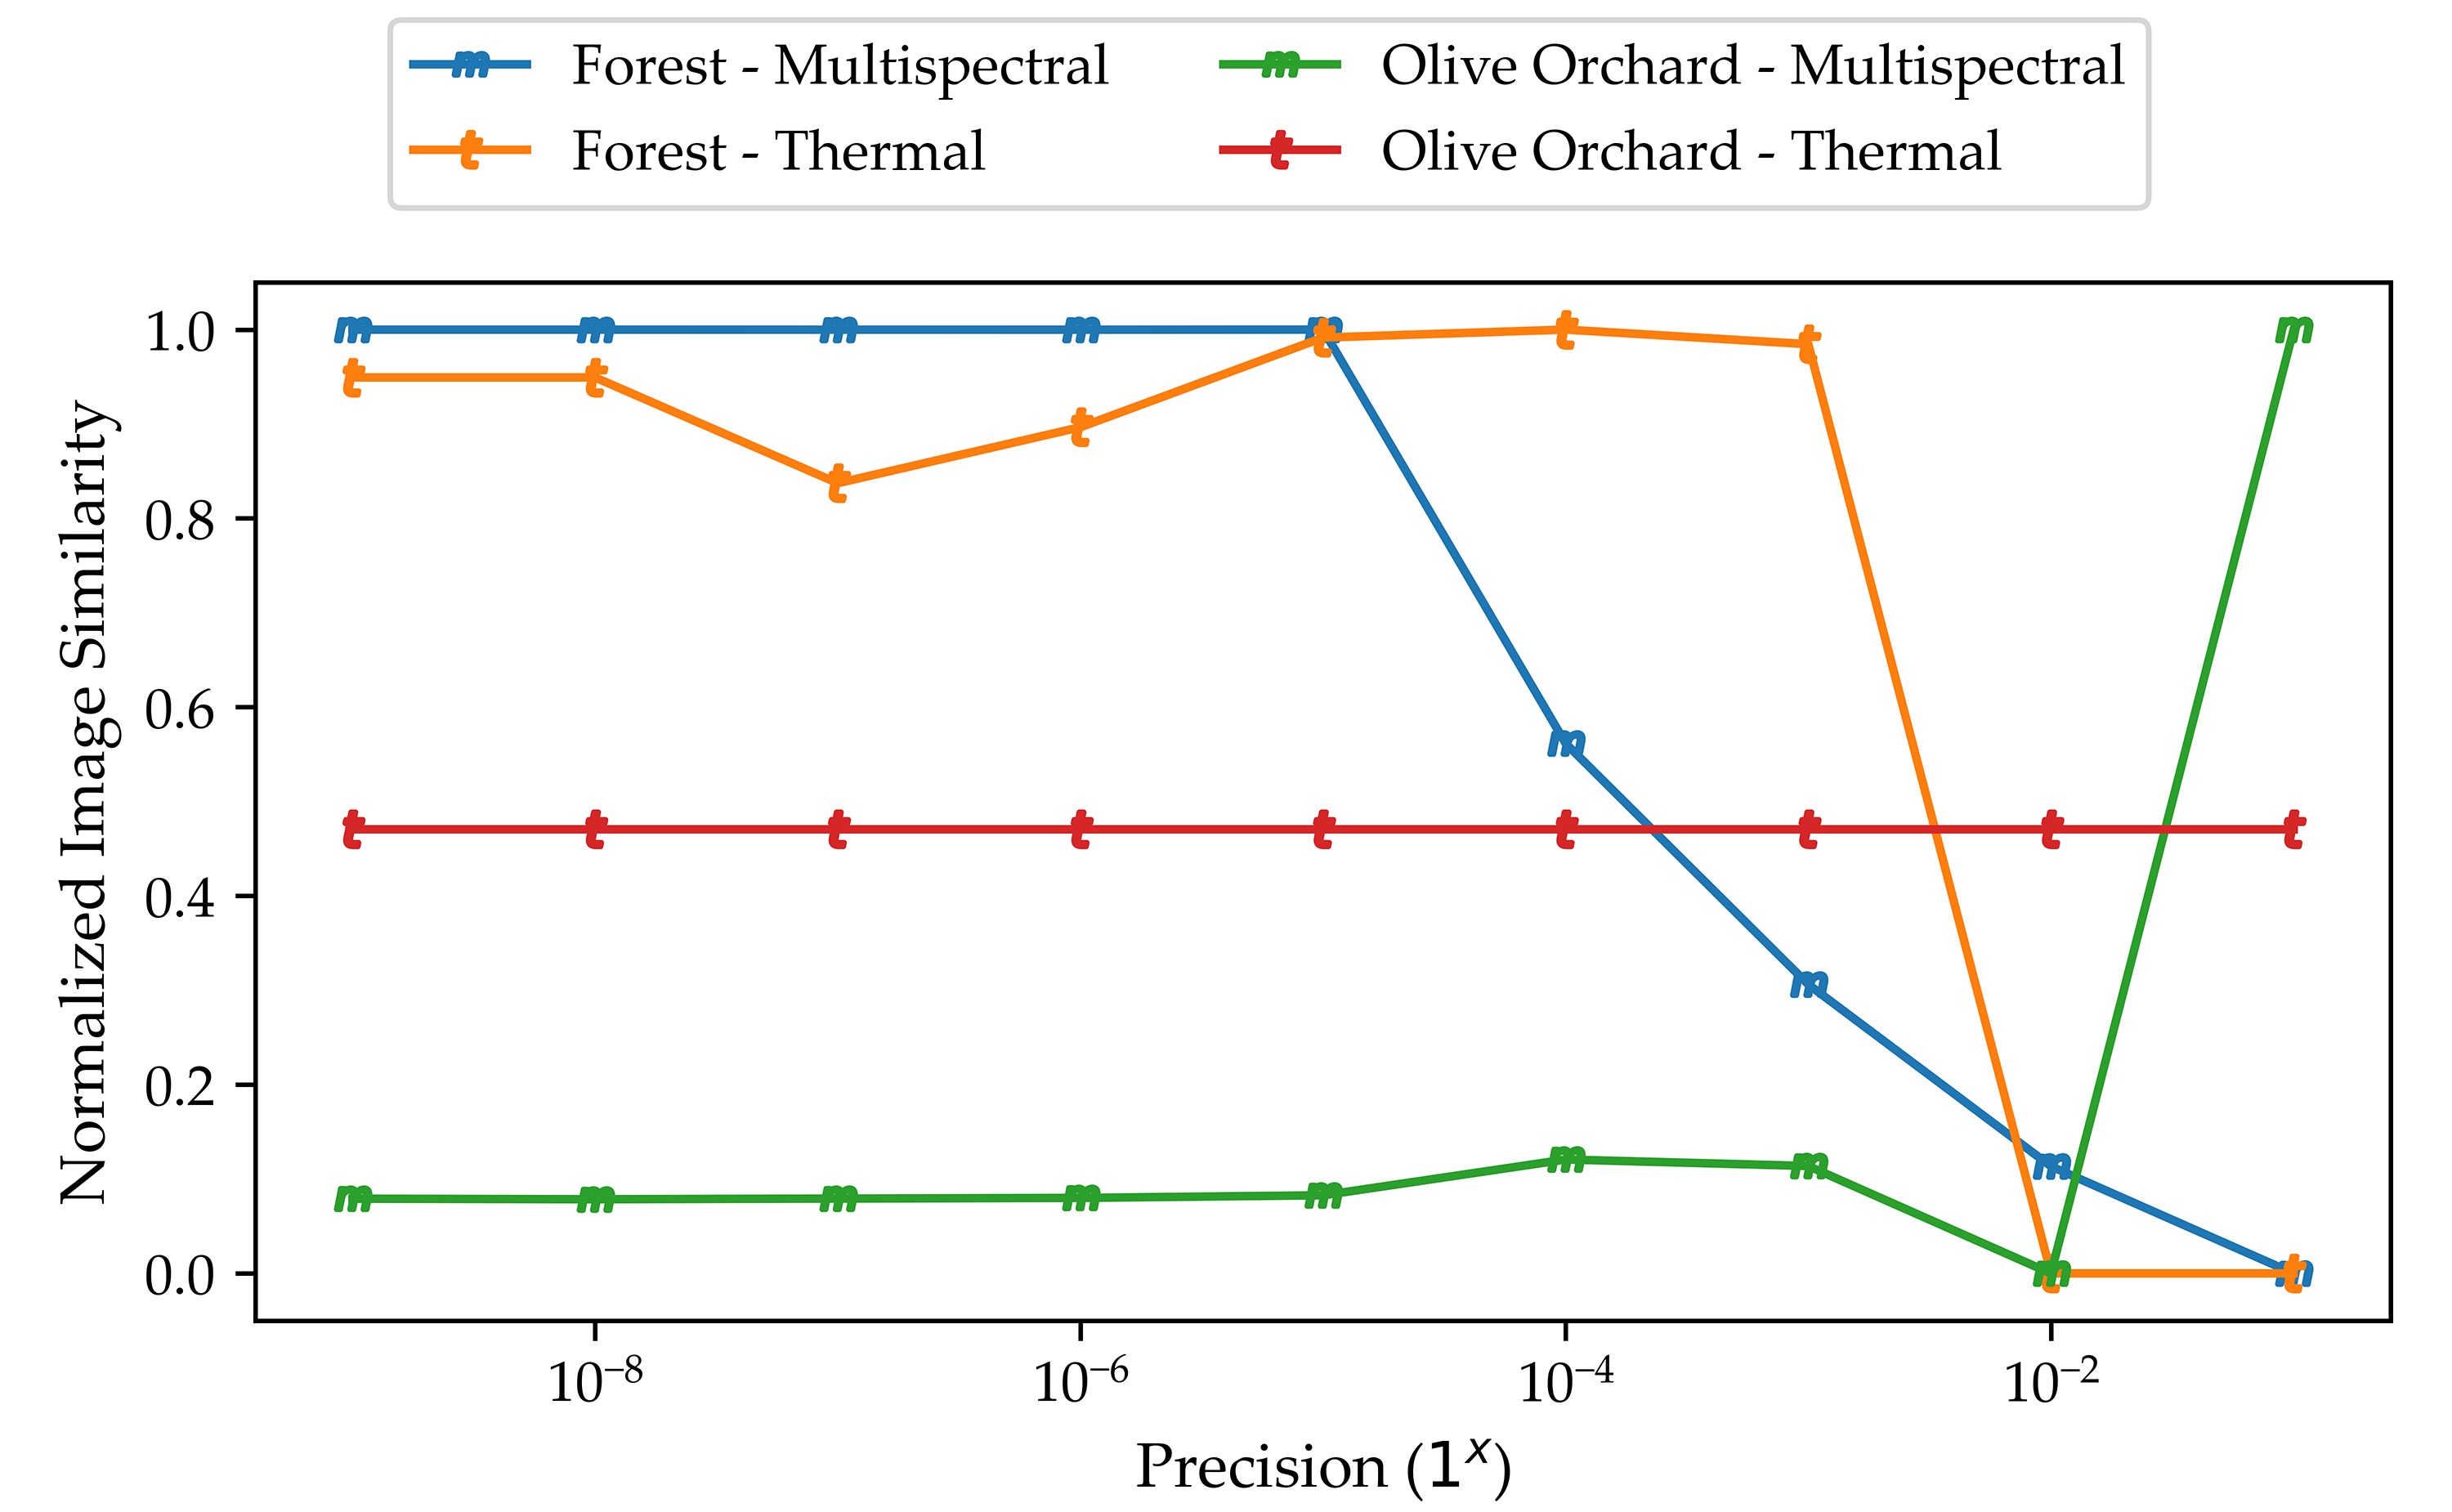
\includegraphics[width=.9\linewidth]{figs/multi_thermal_projection/results/ecc_precision.png}
    \caption{Image similarity measured after performing ECC alignment with a precision equal to $1^x$. Lower values seek the most accurate alignment. The similarity is normalized in [0, 1] for improving the visualization. }
    \label{fig:ecc_precision}
\end{figure}

\subsection{Response time}

First, we compared the response time of commercial solutions against three configurations of our method. The response time is decomposed into three stages: 1) reading the visible point cloud, only for our method, 2) preprocessing stage, including image registration, and 3) reconstruction of the dense point cloud. The second step is related to the procedure of image alignment in commercial software. The results are shown in Figure \ref{fig:occlusion_results_global_time}, and further insight is provided in Table \ref{table:thermal_results} and \ref{table:multispectral_results}. Despite our method reconstructing larger point clouds, the latency is significantly lower than commercial solutions. This difference is further exploited for GPU-based solutions and larger datasets since part of the measured latency comes from the allocation of GPU buffers that can be reused for multispectral layers. Thus, the baseline latency from allocation does not increase with a larger number of images. Accordingly, our sorted GPU solution improves Agisoft Metashape by 77.3\% on average to build thermographic point clouds. The improvement of multispectral reconstruction is 77.26\% with respect to Pix4Dmapper. 

\begin{figure*}[ht]
    \centering
    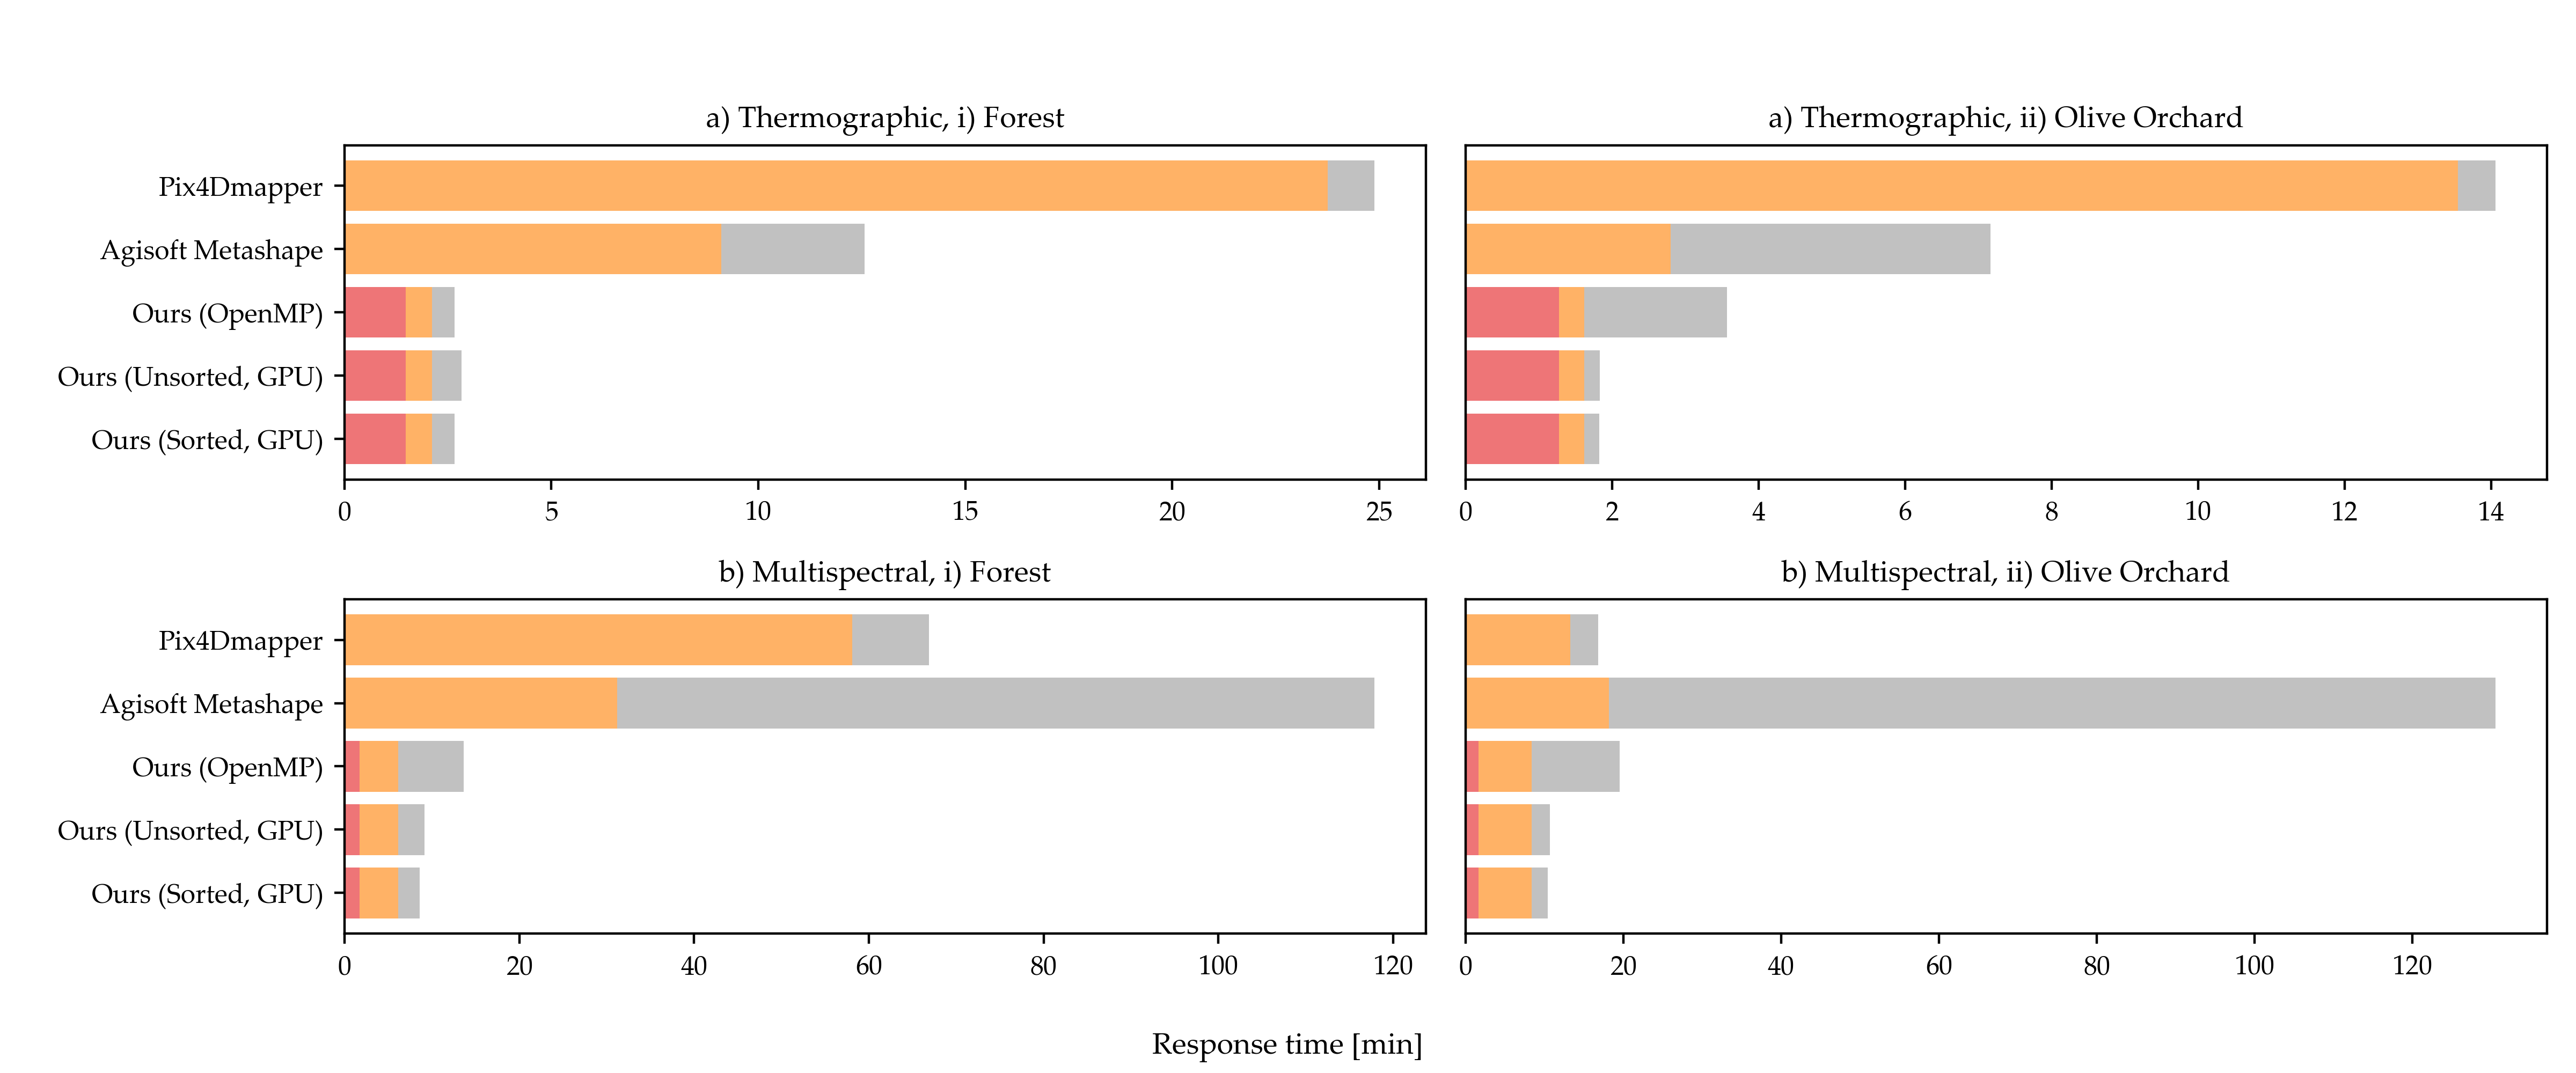
\includegraphics[width=\linewidth]{figs/multi_thermal_projection/results/stacked_global_time.png}
    \caption{Accumulated response time for every data source (1. thermographic and 2. multispectral), study area (A. forestry and b. olive orchard) and solution, including commercial software and configurations of our method. }
    \label{fig:occlusion_results_global_time}
\end{figure*}

The tests were performed with a $z$-buffer with $d \gets 10$, which was shown to balance latency and point cloud dimensionality. Larger values of $d$ involve higher data transfers, while also risking to include background points with foreground data. Otherwise, lower values of $d$ reduce the dimensionality of point clouds at expense of minimizing the latency from data transfers. Based on this, $d \gets 1$ would provide the baseline improvement of ECC method with respect to the recognition of feature points in images to build a sparse point cloud. Both procedures iterate over the whole dataset, whereas the former only evaluates a set of paired images instead of surrounding images. This improvement is considerably lowered for multispectral images since ECC is run up to five times. 

\subsubsection{Comparison of OpenGL and CUDA solutions}

Table \ref{table:cuda_opengl_occlusion_response_time} shows the response time measured from data transfer and the occlusion-aware projection. The single batch configuration loads the whole point cloud in a single buffer if the maximum size of an SSBO is below the maximum allocatable GPU memory. Otherwise, it works as the \textbf{Multiple batches} approach does. On the other hand, the CUDA framework enabled to handle the largest point cloud (271M points) in a single buffer. The reported results were the lowest measured latency from five different tests. The results reported in Table \ref{table:cuda_opengl_occlusion_response_time} and Figure \ref{fig:cuda_opengl_occlusion_response_time} show that compute shaders significantly improve the response time obtained using the traditional rendering pipeline and CUDA. Also, the rendering pipeline offered slightly better results than CUDA for the single-batch workflow, despite being very similar. Regarding the use of multiple batches, both OpenGL-based approaches worsened their performance in comparison with previous tests. In contrast, the CUDA version obtained similar results to the previously measured latency. 

\begin{figure}[htb]
    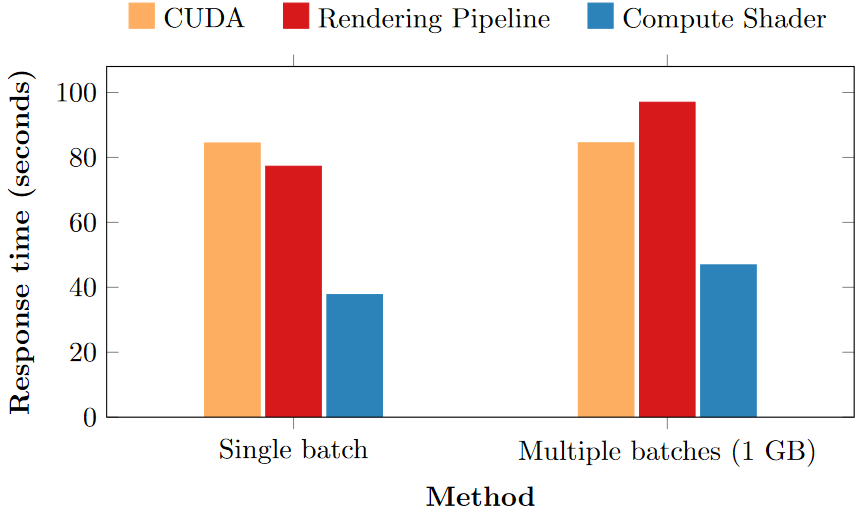
\includegraphics[width=\linewidth]{figs/multi_thermal_projection/results/response_time_cuda_opengl.png}
    \caption{Latency in seconds for OpenGL-based and CUDA approaches for a point cloud of size 271M and 1352 viewpoints).}
    \label{fig:cuda_opengl_occlusion_response_time}
\end{figure}

\renewcommand{\arraystretch}{1.2}
\begin{table*}[hb]
\centering
\caption{Response time of OpenGL and CUDA methodology, including data transfers between CPU and GPU and the core behaviour.}
\label{table:cuda_opengl_occlusion_response_time}
\begin{tabular}{llrrrr}
    \toprule
    \multicolumn{2}{c}{} & \multicolumn{4}{c}{\textbf{Environment}} \\
    \cmidrule{3-6}
    \multicolumn{2}{c}{} & \multicolumn{2}{c}{\textbf{180 cameras}} & \multicolumn{2}{c}{\textbf{1352 cameras}}\\
    \cmidrule{3-6}
    \multicolumn{2}{c}{\textbf{Proposed methods}} & 66M points & 271M points & 66M points & 271M points\\
    \midrule
    \multirow{3}{*}{Single batch} & CUDA & 2.97s & 10.30s & 23.58s & 84.45s\\
    & Rendering pipeline & 2.52s & 10.38s & 20.70s & 77.28s\\
    & Compute shaders & \textbf{1.43s} & \textbf{6.21s} & \textbf{8.90s} & \textbf{37.75s}\\
    \hline
    \multirow{3}{*}{Multiple batches (1 GB)} & CUDA & 3.22s & 11.19s & 25.42s & 84.50s\\
    & Rendering pipeline & 3.71s & 13.35s & 29.15s & 96.99s\\
    & Compute shaders & \textbf{2.57s} & \textbf{7.61s} & \textbf{18.16s} & \textbf{46.90s}\\
    \bottomrule
\end{tabular}
\end{table*}
\renewcommand{\arraystretch}{1}

%As depicted in Figure \arraybackslash, the best configuration of our method outperforms other commercial solutions in terms of both response time and point cloud size. Agisoft Metashape also presents a competitive performance, although the point cloud with maximum quality solely consists of 18M points. On the other hand, the baseline of our method is an RGB point cloud with 98M points. With $d = 10$, we achieve a thermal point cloud with 84M points, whereas the response time is similar to the CUDA-based approach of Agisoft Metashape.

\subsection{Point cloud size and normalized response time}

The proposed method is included as part of a pipeline where dense point clouds of RGB and alternative data sources are jointly reconstructed. In this scenario, the first point cloud is considerably larger than those obtained with imagery of lower resolution and less recognizable features. From this baseline, the number of points of the RGB point cloud is reduced according to their visibility from the whole set of camera viewpoints and the depth buffer's resolution. Still, most of them are preserved and linked to data interpolated from thermal and multispectral imagery in our case study. 

Point clouds reconstructed from multispectral images are dense due to the provided variety of reflectance and the higher number of recognized features. However, the higher sparsity of thermal point clouds is observed in Figure \ref{fig:occlusion_point_cloud_size}. For the thermographic datasets, our method increases the point cloud size by 366.3\% (forest) and 475.52\% (olive orchard) with respect to Agisoft Metashape. In this regard, this commercial solution reconstructs the densest point clouds from the compared software, both for multispectral and thermal imagery. Despite this, it is significantly slower for larger datasets such as the multispectral. For the latter data source, the size increases by 149.89\% (forest) and 141.93\% (olive orchard) also in comparison with Agisoft Metashape.

Previous results based on global latency present a wider gap if they are normalized according to the point cloud's dimensionality. The normalized latency of our best method improves the results of the best commercial solution by 95.51\% and 96.9\% on average for thermal and multispectral images, respectively. 

\newcommand\numExperiments{4}

\renewcommand{\arraystretch}{1.2}
\begin{table*}
    \centering
    \sffamily\footnotesize
    \caption{Numeric results of both commercial solutions and proposed configurations of our method in two different thermal datasets. The global response time is split into reading point cloud (Stage 1), pre-processing (Stage 2) and densification (Stage 3), i.e., generation of a dense point cloud.\\ }
    \label{table:thermal_results}
    \begin{tabular}{l@{\hskip 0.25in}|rrr|r|r|r|r}
    \toprule
    \textbf{Configuration} & \textbf{Stage 1} & \textbf{Stage 2} & \textbf{Stage 3} & \textbf{Latency} & \textbf{Latency/point} & \textbf{Point cloud size} & \textbf{Matching}\\
    \cmidrule{1-8}
    \multicolumn{8}{c}{Thermal Dataset 1 (Forestry)}\\
    \cmidrule{1-8}
    Pix4Dmapper & - & 23.76 \si{\minute} & 1.13 \si{\minute} & 24.89 \si{\minute} & 449.08 \si{\micro\second}/point & 3,325,454 points & 98\%\\
    Agisoft Metashape & - & \textbf{9.10} \si{\minute} & 3.47 \si{\minute} & 12.57 \si{\minute} & 35.05 \si{\micro\second}/point & 21,514,286 points & 62.95\%\\
    \cmidrule{1-8}
    OpenMP, No Sort & \multirow{\numExperiments}{*}{1.48 \si{\minute}} & \multirow{\numExperiments}{*}{\textbf{0.64 \si{\minute}}} & 9.77 \si{\minute} & 11.89 \si{\minute} & 6.90 \si{\micro\second}/point & \multirow{\numExperiments}{*}{\textbf{100,322,449 points}} & \multirow{\numExperiments}{*}{\textbf{99.287\%}}\\
    GPU, No Sort & & & 0.71 \si{\minute} & 2.83 \si{\minute} & 1.69 \si{\micro\second}/point & &\\
    GPU, Global Sort & & & \textbf{0.546 \si{\minute}} & \textbf{2.666 \si{\minute}} & \textbf{1.594 \si{\micro\second}/point} & &\\
    %Ours - GPU, Shuffle Sort & & & \textbf{0.543 \si{\minute}} & \textbf{2.663 \si{\minute}} & \textbf{1.592 \si{\micro\second}/point} & &\\
    \bottomrule
    \toprule
    \multicolumn{8}{c}{Thermal Dataset 2 (Olive orchard)}\\
    \cmidrule{1-8}
    Pix4Dmapper & - & 13.55 \si{\minute} & 0.51 \si{\minute} & 14.06 \si{\minute} & 388.92 \si{\micro\second}/point & 2,169,058 points & 90\%\\
    Agisoft Metashape & - & \textbf{2.80} \si{\minute} & 4.37 \si{\minute} & 7.17 \si{\minute} & 32.79 \si{\micro\second}/point & 13,117,583 
     points & \textbf{99.39\%}\\
    \cmidrule{1-8}
    OpenMP, No Sort & \multirow{\numExperiments}{*}{1.28 \si{\minute}} & \multirow{\numExperiments}{*}{\textbf{0.34 \si{\minute}}} & 1.95 \si{\minute} & 3.57 \si{\minute} & 2.83 \si{\micro\second}/point & \multirow{\numExperiments}{*}{\textbf{75,494,967 points}} & \multirow{\numExperiments}{*}{89.75\%}\\
    GPU, No Sort & & & 0.217 \si{\minute} & 1.837 \si{\minute} & 1.459 \si{\micro\second}/point & &\\
    GPU, Global Sort & & & \textbf{0.208 \si{\minute}} & \textbf{1.828 \si{\minute}} & \textbf{1.452 \si{\micro\second}/point} & &\\
    %Ours - GPU, Shuffle Sort & & & \textbf{0.207 \si{\minute}} & \textbf{1.827 \si{\minute}} & \textbf{1.452 \si{\micro\second}/point} & &\\
    \bottomrule
    \end{tabular}
\end{table*}
\renewcommand{\arraystretch}{1}

\renewcommand{\arraystretch}{1.2}
\begin{table*}
    \centering
    \footnotesize
    \caption{Continuation of Table \ref{table:thermal_results} for multispectral imagery.\\ }
    \label{table:multispectral_results}
    \begin{tabular}{l@{\hskip 0.25in}|rrr|r|r|r|r}
    \toprule
    \textbf{Configuration} & \textbf{Stage 1} & \textbf{Stage 2} & \textbf{Stage 3} & \textbf{Latency} & \textbf{Latency/point} & \textbf{Point cloud size} & \textbf{Matching}\\
    \cmidrule{1-8}
    \multicolumn{8}{c}{Multispectral Dataset 1 (Forestry)}\\
    \cmidrule{1-8}
    Pix4Dmapper & - & 58.11 \si{\minute} & \textbf{8.76} \si{\minute} & 66.87 \si{\minute} & 398.35 \si{\second}/point & 10,071,939 points & 97\%\\
    Agisoft Metashape & - & \textbf{31.22} \si{\minute} & 86.64 \si{\minute} & 117.86 \si{\minute} & 165.49 \si{\micro\second}/point & 42,731,004 points & 67.74\%\\
    \cmidrule{1-8}
    OpenMP, No Sort & \multirow{\numExperiments}{*}{1.71 \si{\minute}} & \multirow{\numExperiments}{*}{\textbf{4.45 \si{\minute}}} & 7.50 \si{\minute} & 13.66 \si{\minute} & 7.67 \si{\micro\second}/point & \multirow{\numExperiments}{*}{\textbf{106,780,612 points}} & \multirow{\numExperiments}{*}{\textbf{100\%}}\\
    GPU, No Sort & & & 2.99 \si{\minute} & 9.15 \si{\minute} & 5.14 \si{\micro\second}/point & &\\
    GPU, Global Sort & & & \textbf{2.42 \si{\minute}} & \textbf{8.58 \si{\minute}} & \textbf{4.82 \si{\micro\second}/point} & &\\
    %Ours - GPU, Shuffle Sort & & & \textbf{2.40 \si{\minute}} & \textbf{8.56 \si{\minute}} & \textbf{4.80 \si{\micro\second}/point} & &\\
    \bottomrule
    \toprule
    \multicolumn{8}{c}{Multispectral Dataset 2 (Olive orchard)}\\
    \cmidrule{1-8}
    Pix4Dmapper & - & \textbf{13.3} \si{\minute} & \textbf{3.5} \si{\minute} & 16.8 \si{\minute} & 92.56 \si{\micro\second}/point & 10,889,523 points & \textbf{100\%}\\
    Agisoft Metashape & - & 18.15 \si{\minute} & 112.36 \si{\minute} & 130.51 \si{\minute} & 150,52 \si{\micro\second}/point & 52,021,396 points & \textbf{100\%}\\
    \cmidrule{1-8}
    OpenMP, No Sort & \multirow{\numExperiments}{*}{1.67 \si{\minute}} & \multirow{\numExperiments}{*}{\textbf{6.69} \si{\minute}} & 11.19 \si{\minute} & 19.55 \si{\minute} & 9.32 \si{\micro\second}/point & \multirow{\numExperiments}{*}{\textbf{125,857,793 points}} & \multirow{\numExperiments}{*}{99.934 \%}\\
    GPU, No Sort & & & 2.31 \si{\minute} & 10.67 \si{\minute} & 5.08 \si{\micro\second}/point & &\\
    GPU, Global Sort & & & \textbf{2.08 \si{\minute}} & \textbf{10.44 \si{\minute}} & \textbf{4.97 \si{\micro\second}/point} & &\\
    %Ours - GPU, Shuffle Sort & & & 2.09 \si{\minute} & 10.45 \si{\minute} & 4.98 \si{\micro\second}/point & &\\
    \bottomrule
    \end{tabular}
\end{table*}
\renewcommand{\arraystretch}{1}

\newpage
\subsection{Overall comparison}

\begin{marginfigure}[.1cm]
    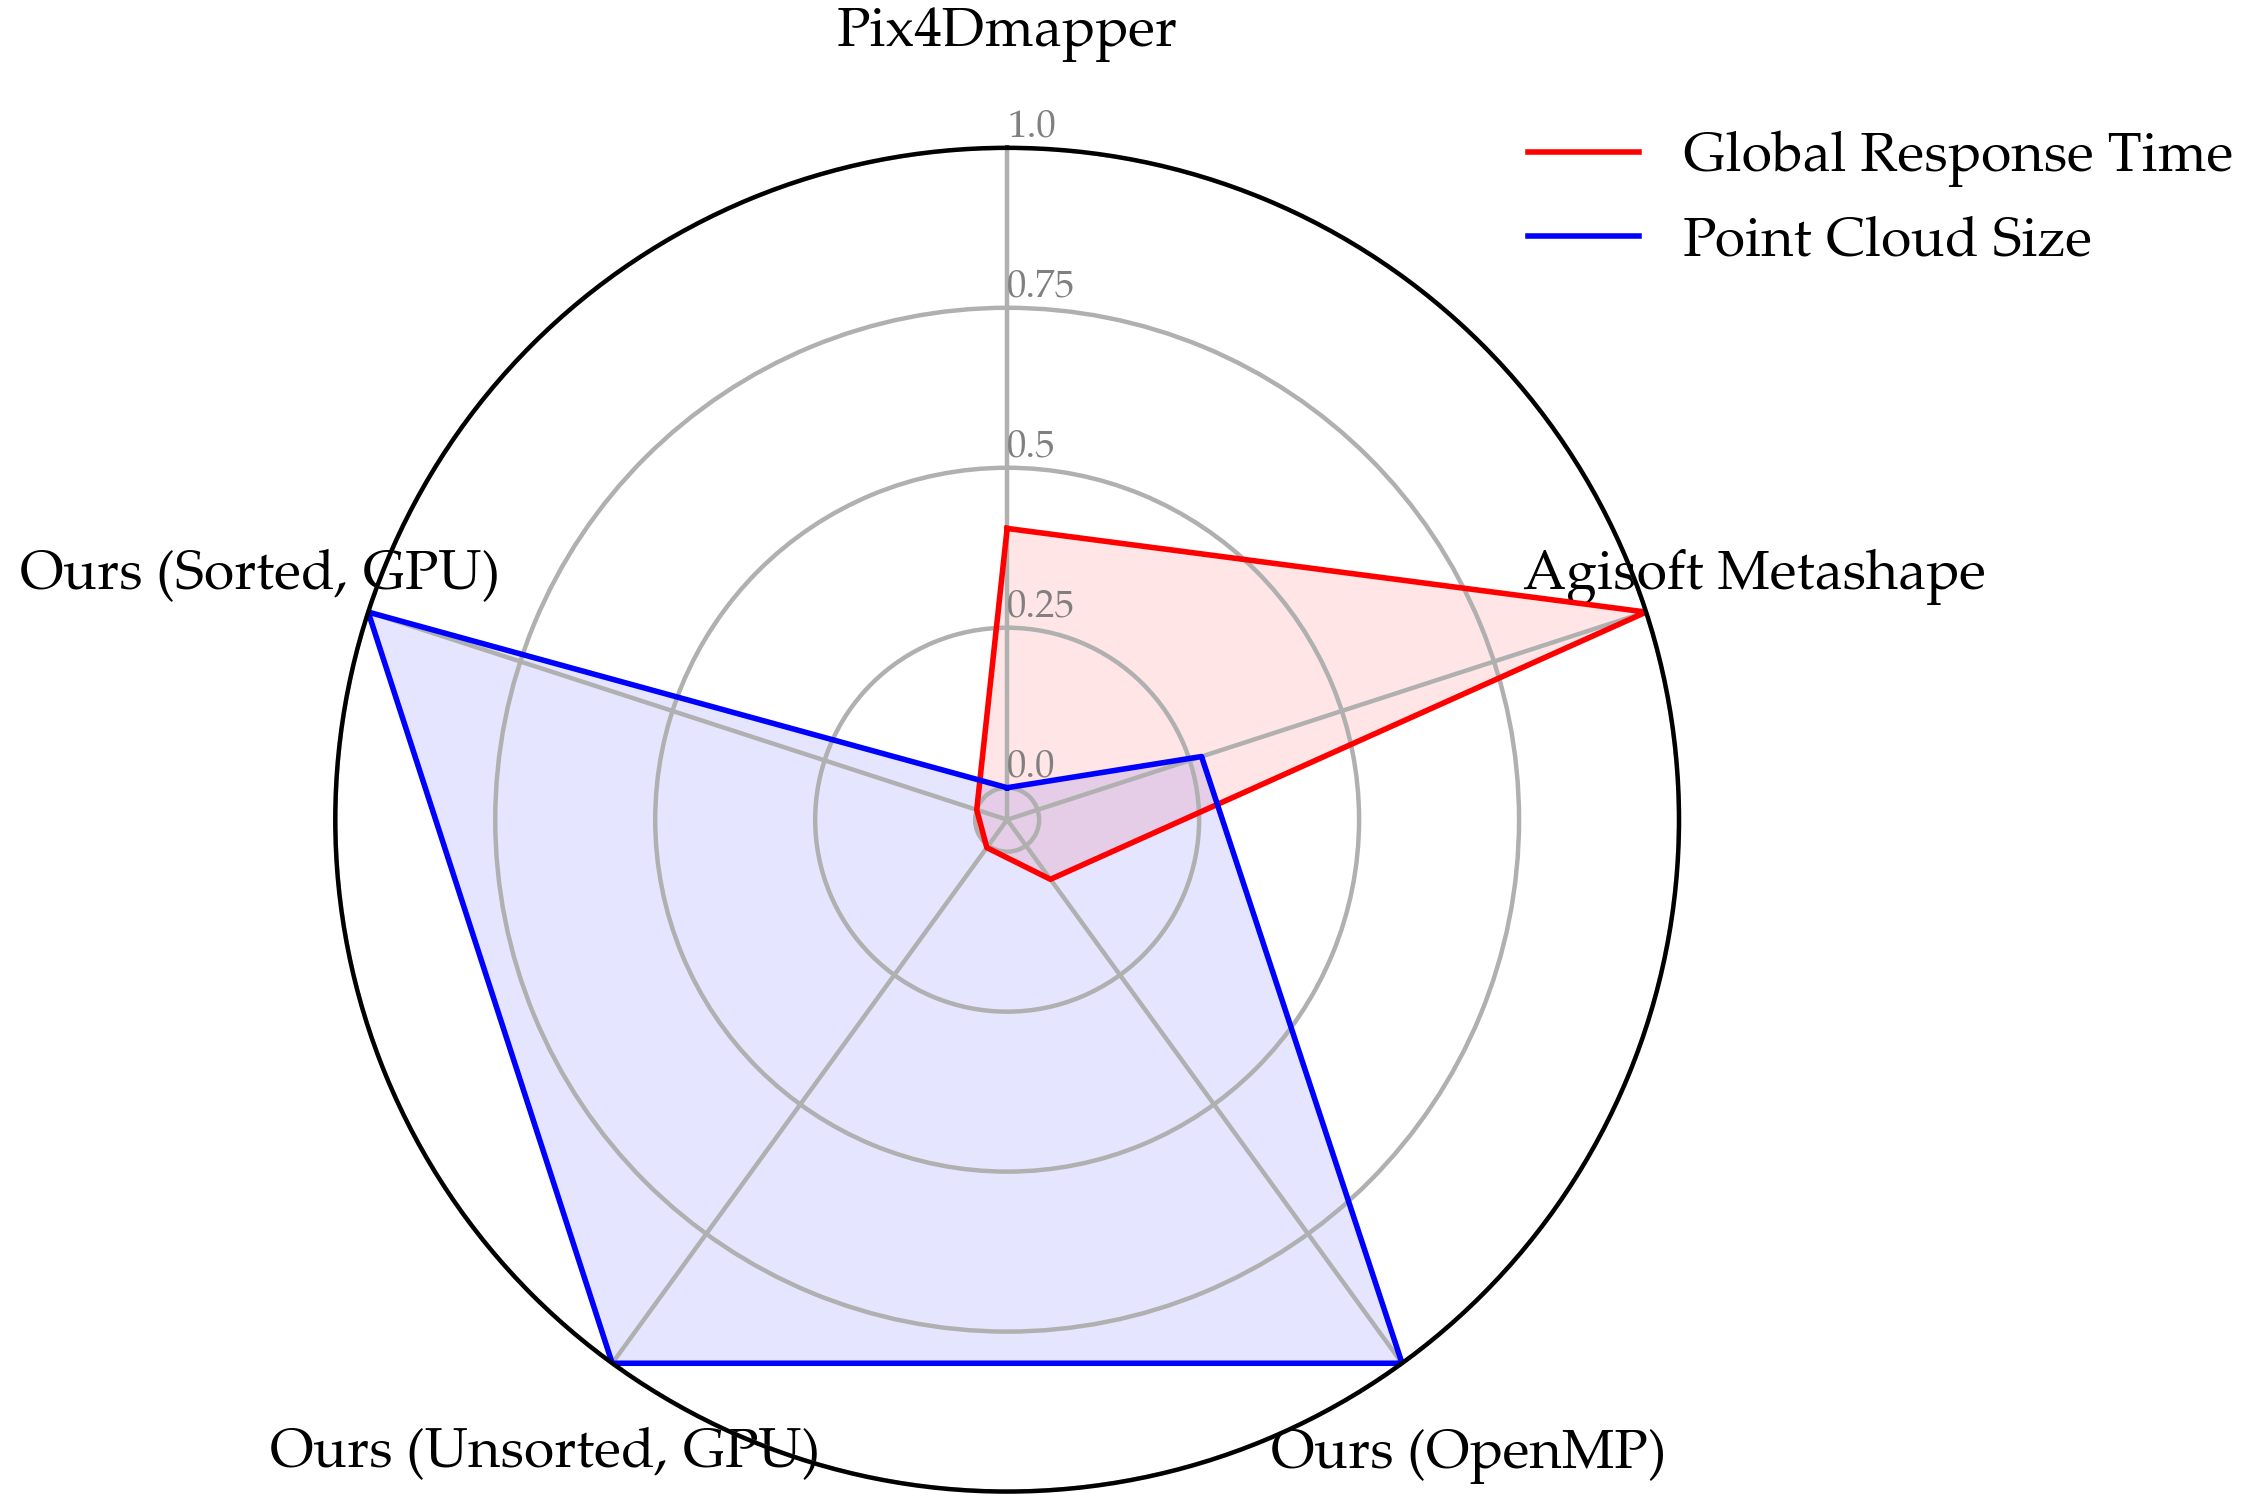
\includegraphics[width=\linewidth]{figs/multi_thermal_projection/results/normalized_features.png}
    \caption{Average response time and point cloud size obtained by commercial software and three versions of the proposed method.}
    \label{fig:occlusion_normalized_features}
\end{marginfigure}
The results of the four datasets and the five compared methods are summarized in Figure \ref{fig:occlusion_normalized_features}. The global latency and point cloud size features are normalized in $[0, 1]$. The first feature must be minimized, whereas the second one ought to be maximized to provide better visualization and details of the target dataset. According to this figure, the three proposed methods present an outstanding performance in terms of response time and point cloud dimensionality. These are followed by Agisoft Metashape, which is considerably slower, albeit generating larger results than the last alternative, Pix4Dmapper.

\subsection{Data shuffling in GPU}

\begin{figure}
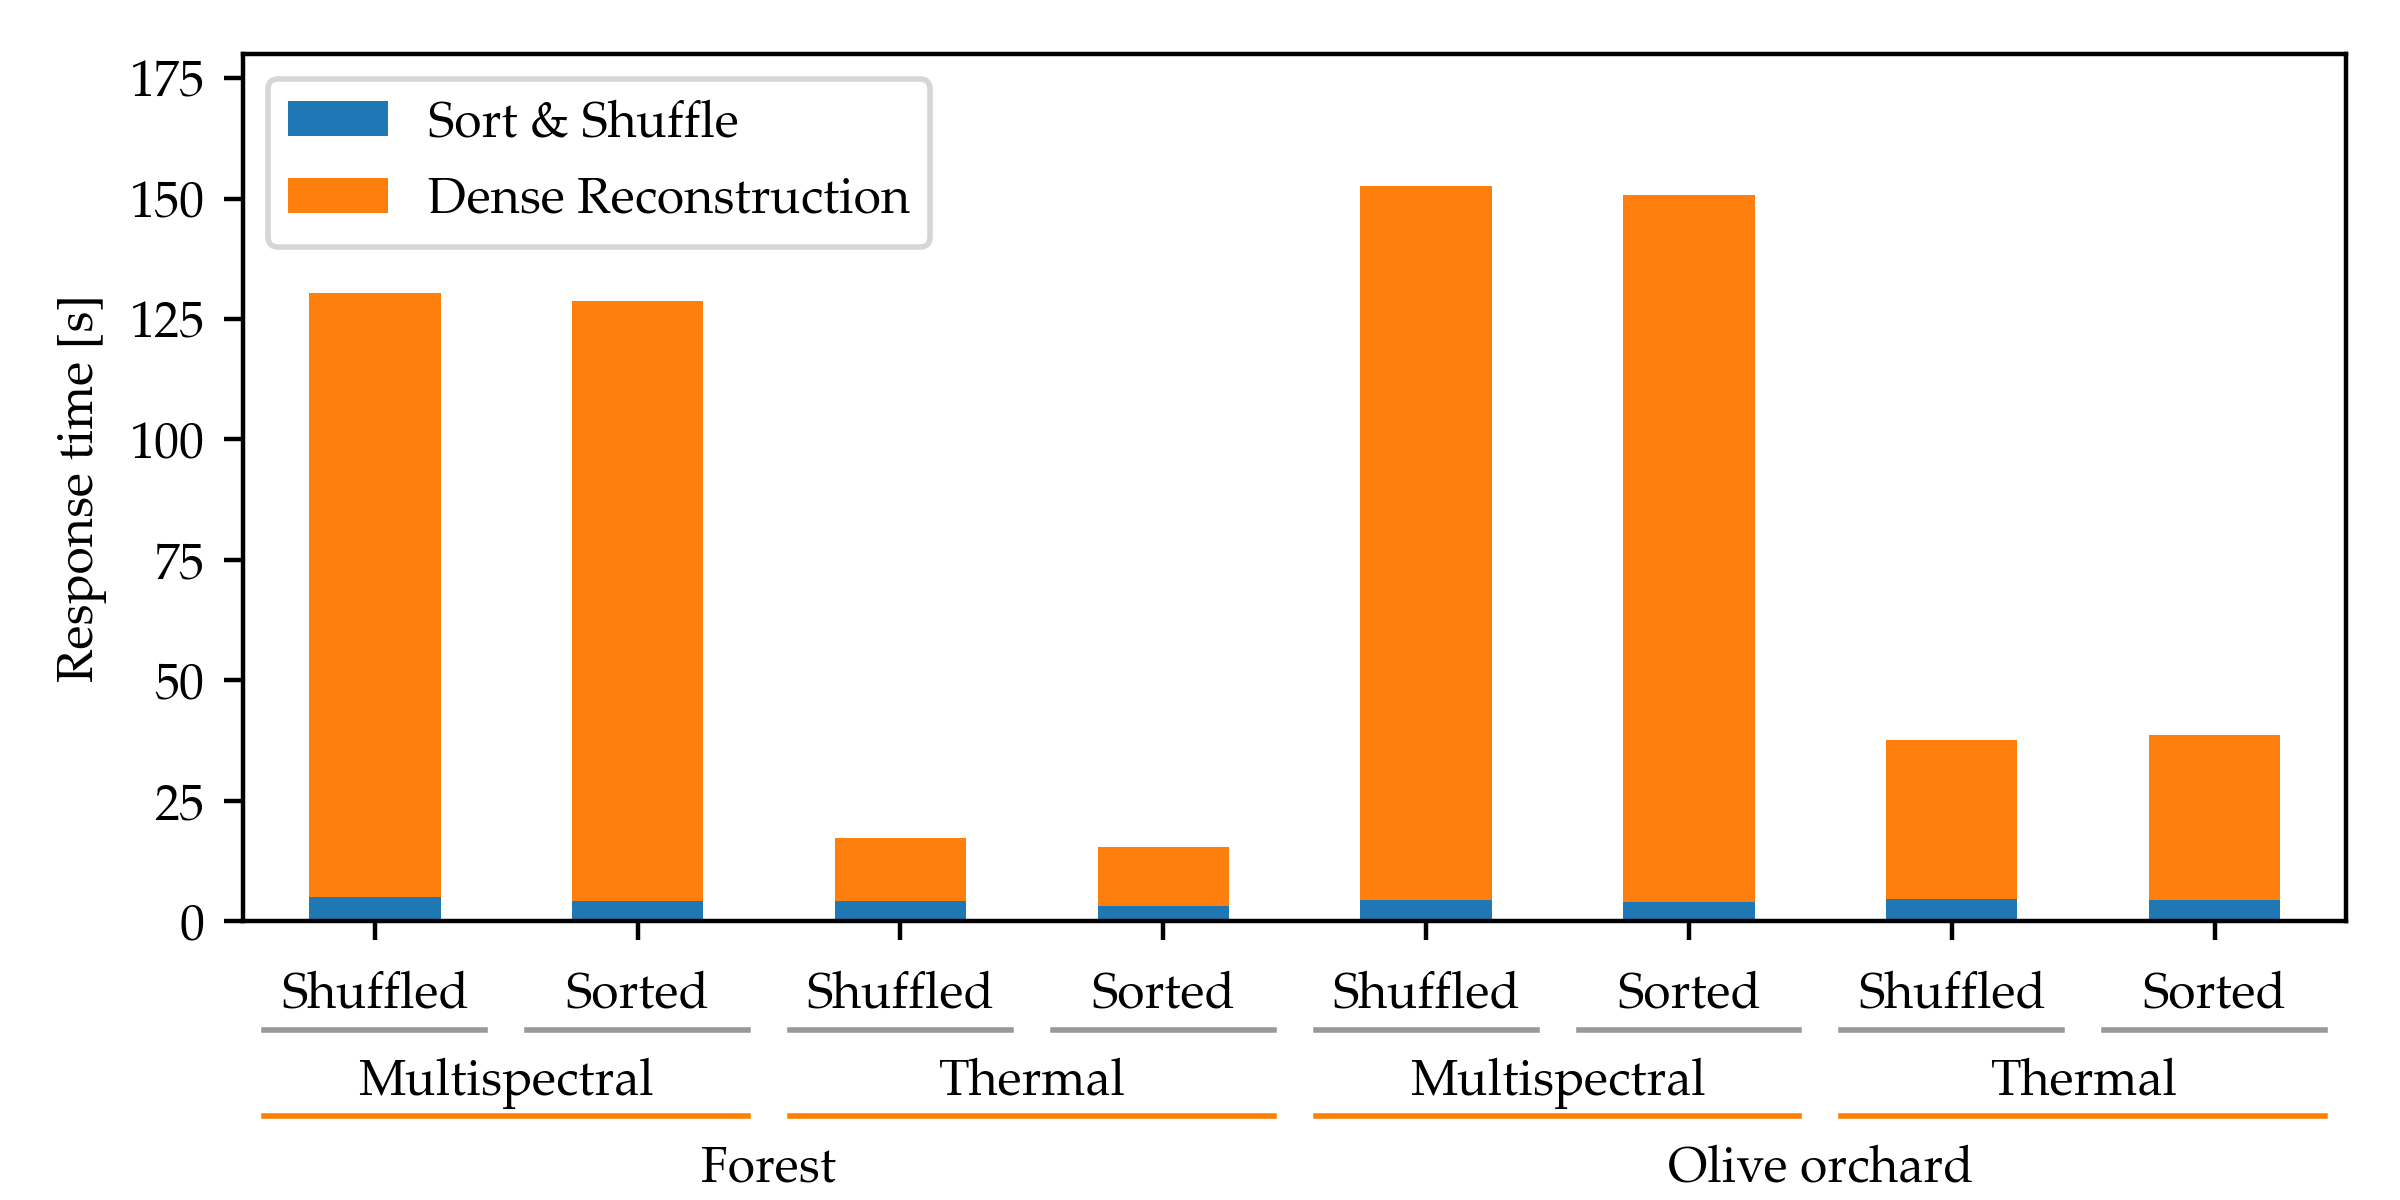
\includegraphics[width=\linewidth]{figs/multi_thermal_projection/results/stacked_stage_response_time.png}
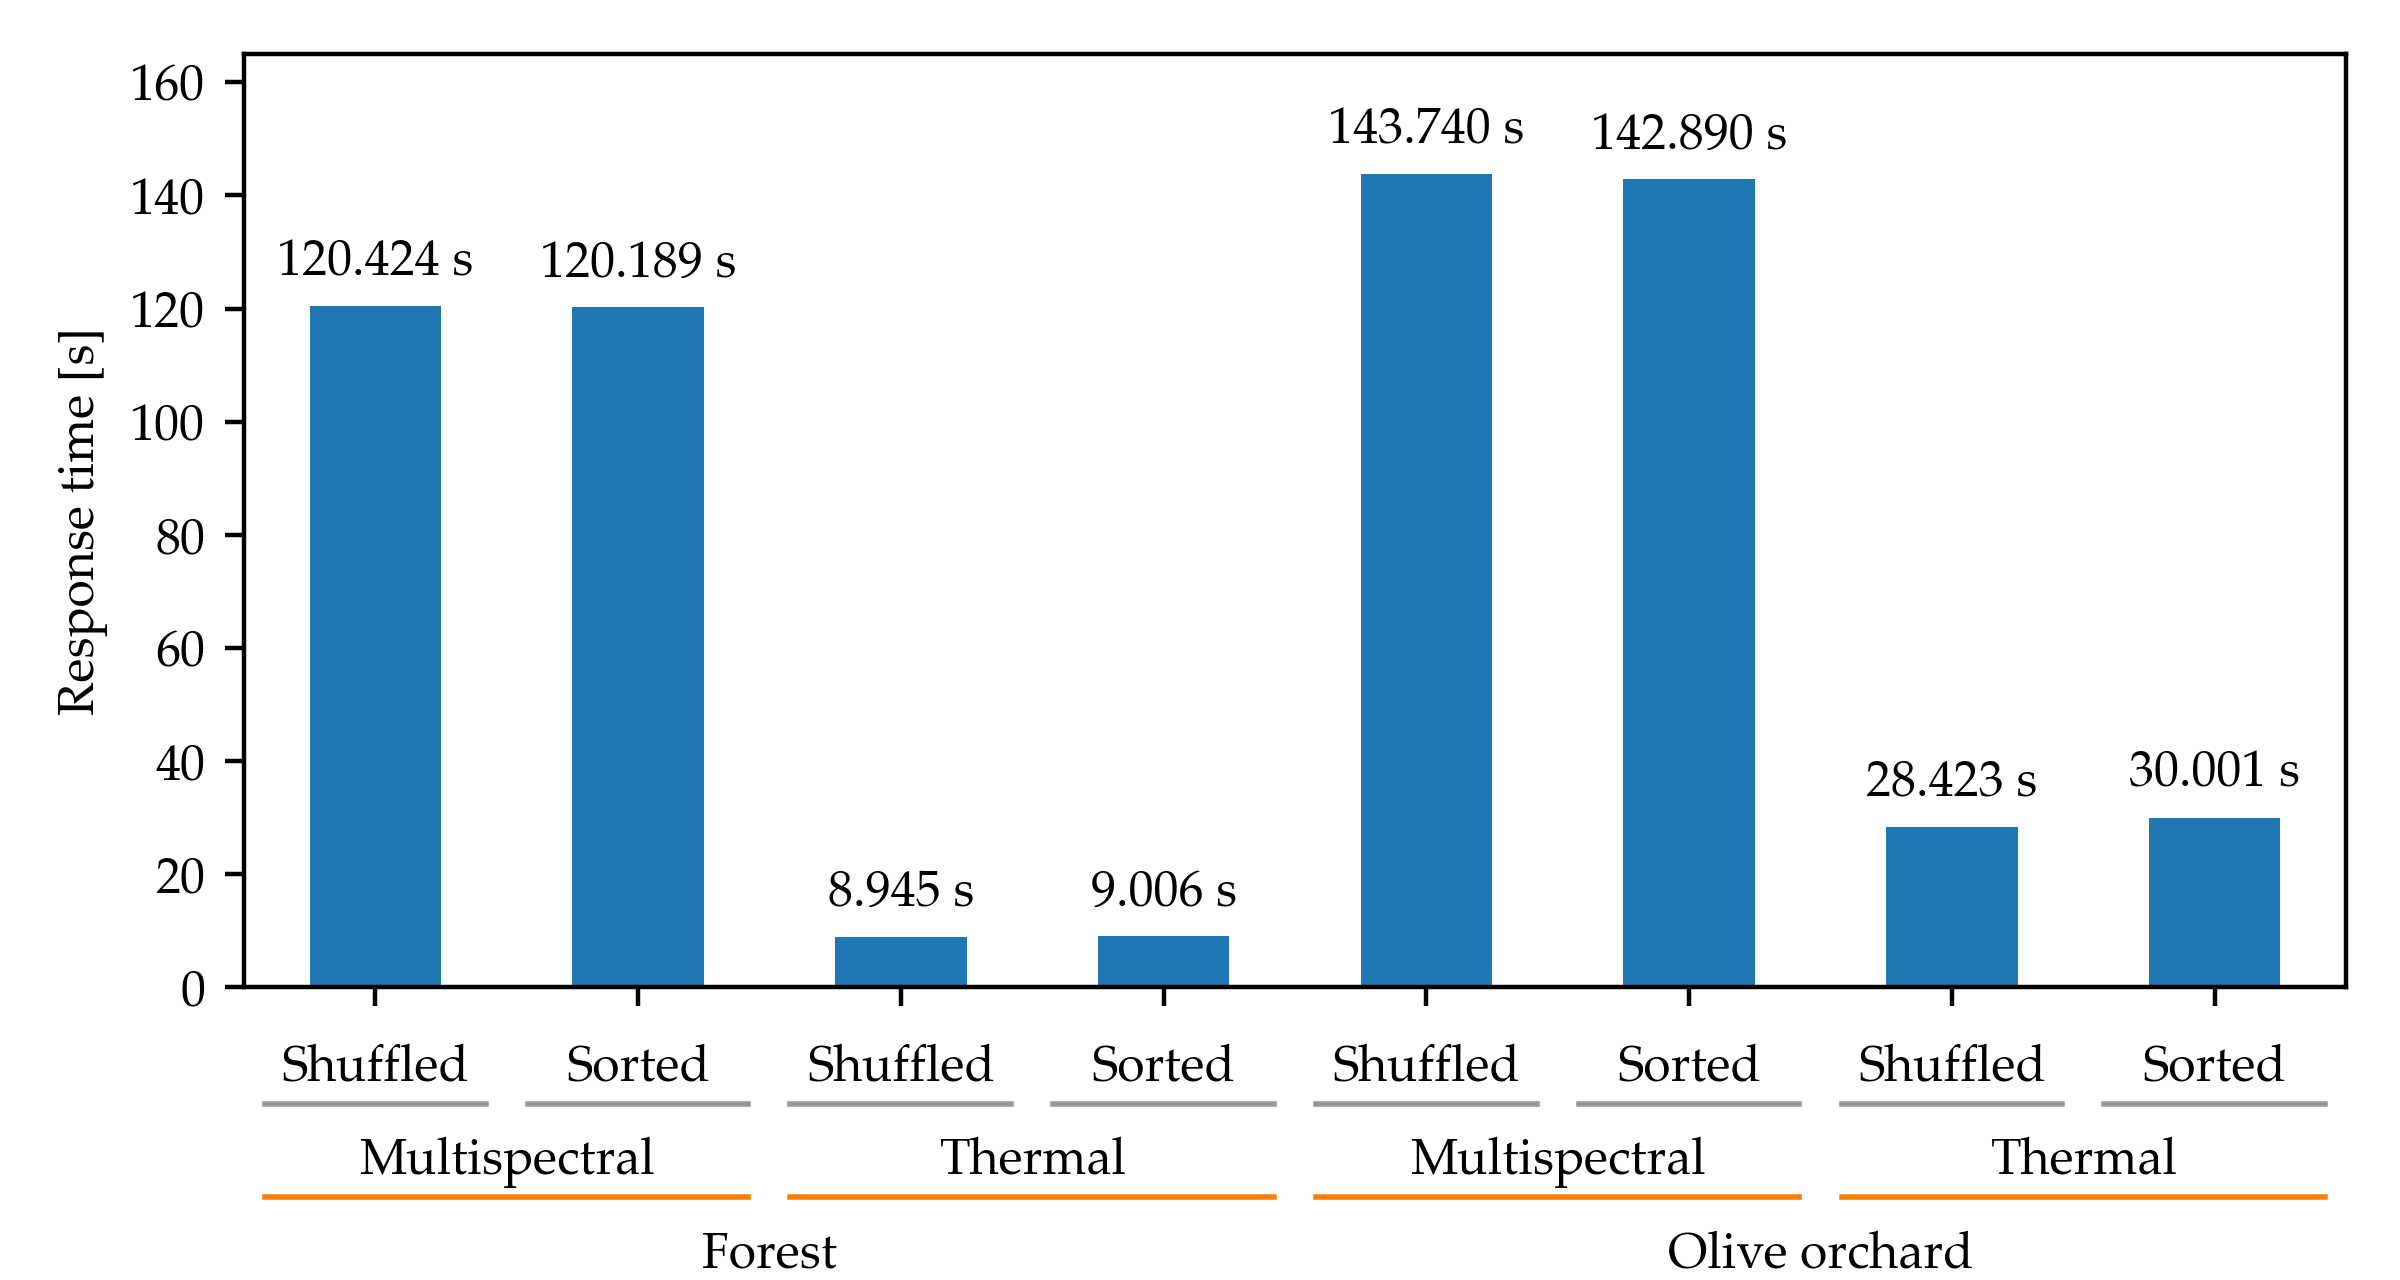
\includegraphics[width=\linewidth]{figs/multi_thermal_projection/results/shuffled_response_time.png}
\caption{Comparison of performance of the dense reconstruction stage using sorted \& shuffled data and globally sorted data. The first image compares the overall latency of the dense reconstruction, whereas the second image only compares the projection procedure.}
\label{fig:shuffle_comparison}
\end{figure}

\begin{figure*}
    \ContinuedFloat
    \centering
    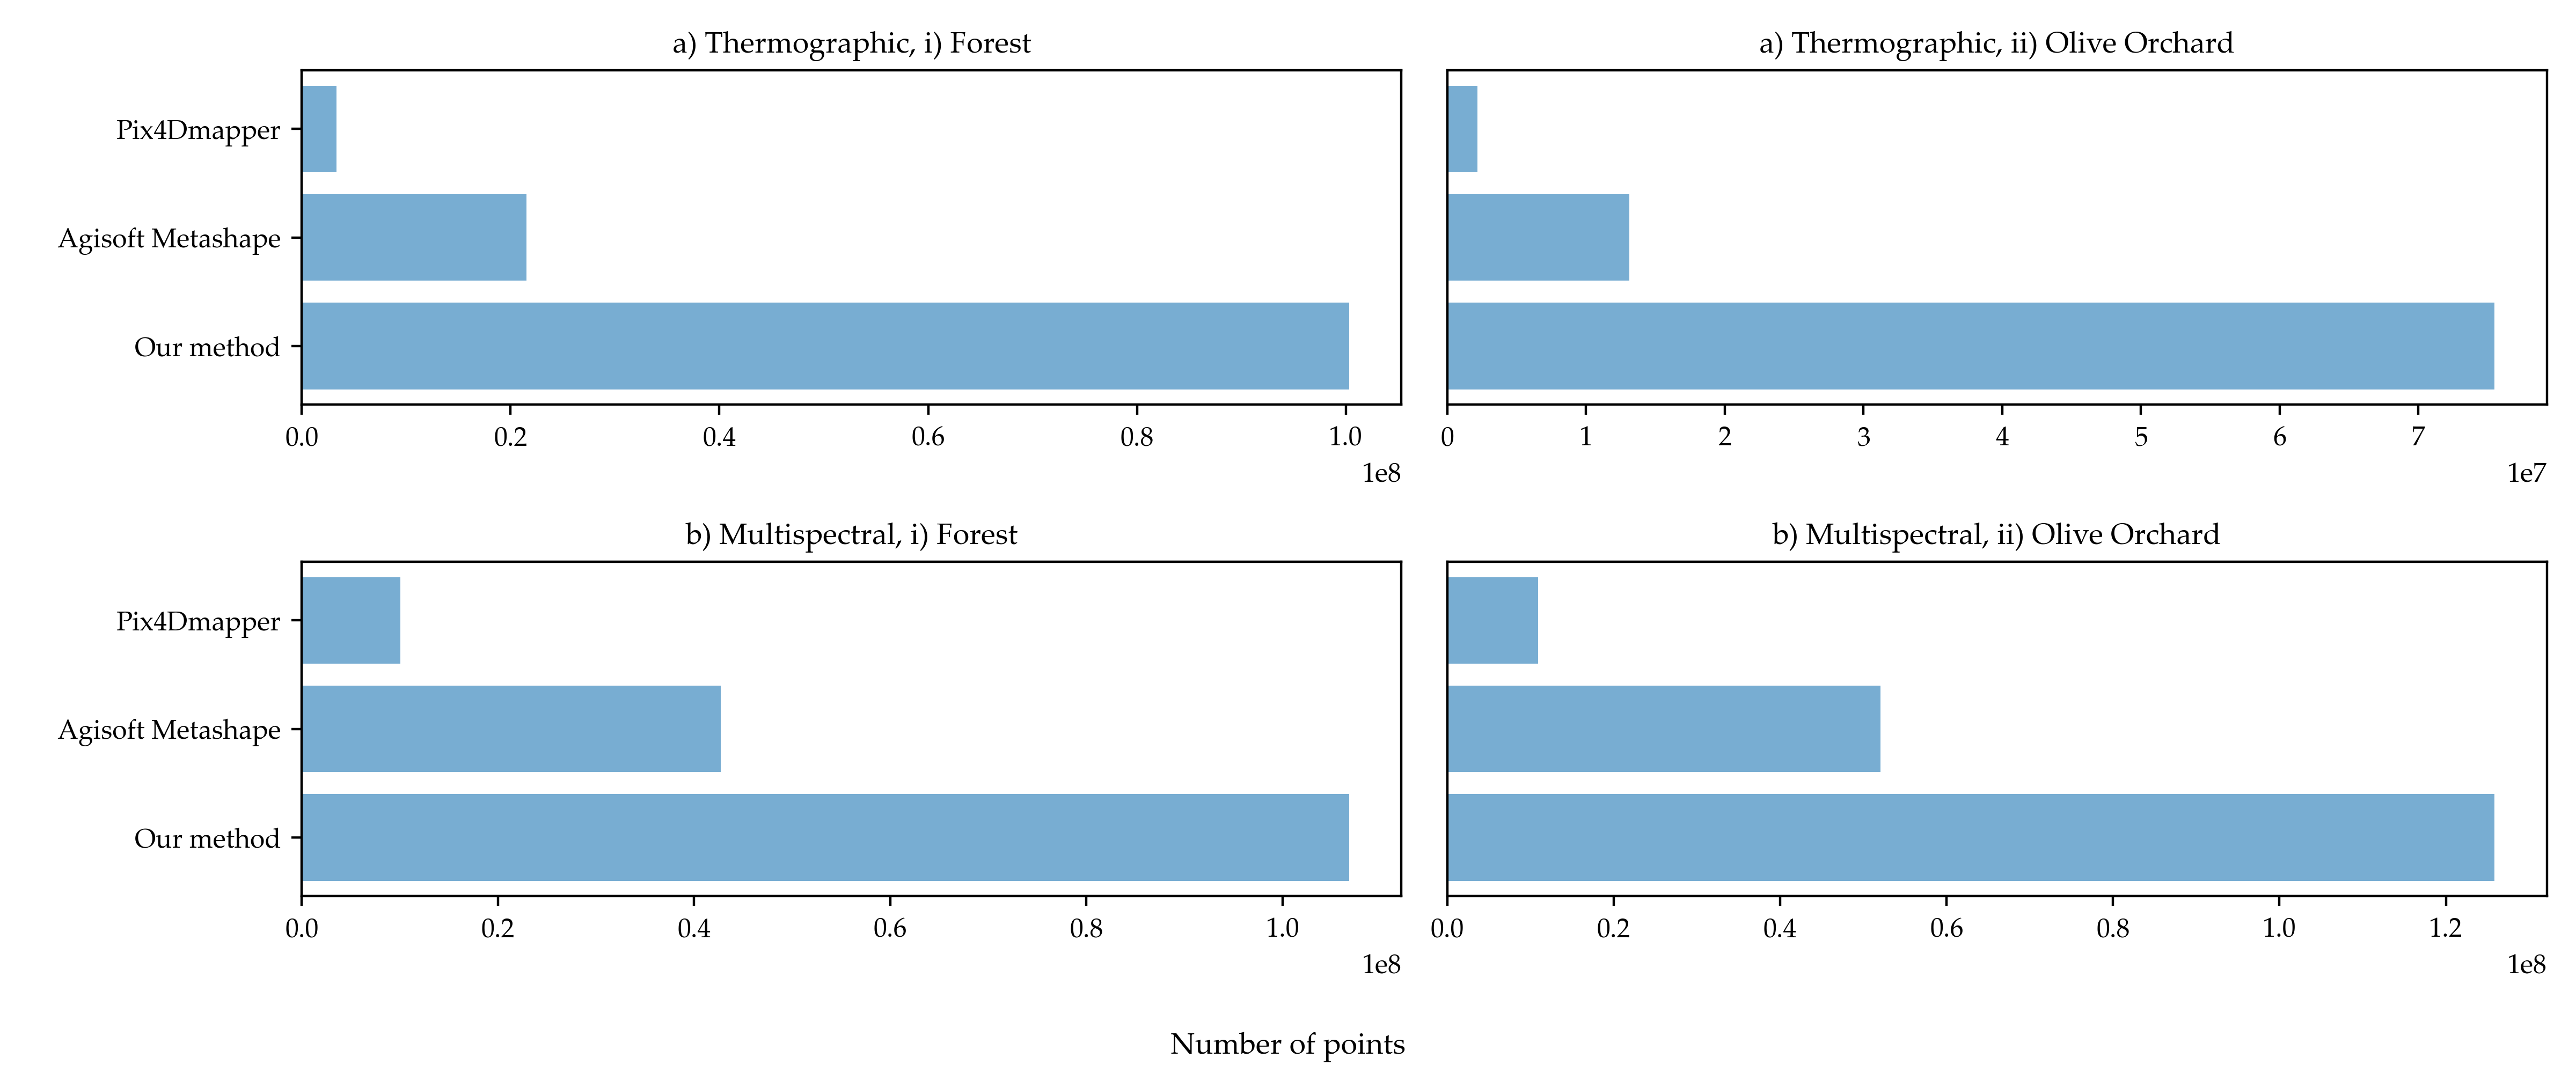
\includegraphics[width=\linewidth]{figs/multi_thermal_projection/results/point_cloud_size.png}
    \caption{Continuation of Figure \ref{fig:occlusion_results_global_time} on the dimensionality of the reconstructed point clouds. }
    \label{fig:occlusion_point_cloud_size}
\end{figure*}

As stated by previous work \cite{schutz_rendering_2021, kerbl_effective_2017}, specific GPU patterns are used by manufacturers to distribute the workload among thread groups. This knowledge can help to further reduce the latency of GPU-based solutions, in comparison with globally sorted point clouds. Thus, the objective is to shuffle points in batches to balance the workload of every workgroup. As the outcome of a batch is expected to depend on the camera viewpoint, the data shuffling ought to help to reduce latency by distributing visible and non-visible points. To this end, we conducted a comparison of data shuffled or not after being sorted, with groups of size $g \gets 32$. The results are depicted in Figure \ref{fig:shuffle_comparison} by splitting the latency into the Sort \& Shuffle and Reconstruction stages. Numeric results are also annotated in Table \ref{table:shuffling_results}.

\renewcommand{\arraystretch}{1.2}
\begin{table*}
    \footnotesize
    \centering
    \caption{Latency of the first two stages if 1) it is the first load or 2) binary data has already been stored as a result of a previous load. }
    \label{table:shuffling_results}
    
    \begin{tabular}{l@{\hskip 0.15in}|cc|cc}
    \toprule
     & \multicolumn{2}{c}{Global sort} & \multicolumn{2}{c}{Shuffled sort ($g \gets 32$)}\\
    \cmidrule{1-5}
    \textbf{Dataset} & Point cloud sort & Dense reconstruction &  Point cloud sort & Dense reconstruction\\
    \cmidrule{1-5}
    a) Thermal, i) Forest & \textbf{0.071 \si{\minute}} & 0.500 \si{\minute}
    & 0.076 \si{\minute} & \textbf{0.473} \si{\minute}\\
    \cmidrule{1-5}
    a) Thermal, ii) Olive orchard & \textbf{0.052 \si{\minute}} & 0,150 \si{\minute}
    & 0.052 \si{\minute} & \textbf{0.149 \si{\minute}}\\
    \cmidrule{1-5}
    b) Multispectral, i) Forest & \textbf{0.065 \si{\minute}} & \textbf{2.381 \si{\minute}}
    & 0.074 \si{\minute} & 2.395 \si{\minute}\\
    \cmidrule{1-5}
    b) Multispectral, ii) Olive orchard & \textbf{0.071 \si{\minute}} & \textbf{2.003 \si{\minute}}
    & 0.082 \si{\minute} & 2.007 \si{\minute}\\
    \bottomrule
    \end{tabular}
\end{table*}
\renewcommand{\arraystretch}{1}

To provide a better insight into the data shuffling, the second image shows only the response time from the dense reconstruction. The shuffled ordering also involves global sorting prior to organizing the point cloud into batches. Thus, the Sort \& Shuffle procedure is more time-consuming than solely sorting. Accordingly, the summed response time of the Shuffled version is higher for every configuration whether we include both stages. Otherwise, the results offer slight changes whether only the reconstruction stage is considered. It is observed that data shuffling effectively helps to reduce latency in smaller point clouds (thermographic), whereas larger point clouds worsen the latency obtained by the global sort. Unlike previous studies, the proposed case study is very unbalanced for individual viewpoints. From hundreds of millions of points, only a few million are visible from a camera viewpoint. Thus, the workload balancing was not effective. Even if so, the Shuffle stage increases the latency for a one-time process, thus making it not worth it. Instead, real-time processes such as rendering are more likely to take advantage of this technique.

\subsection{Visual results}

Table \ref{table:visual_results} shows the rendering of multispectral and thermographic point clouds obtained by the three compared solutions. In this regard, both commercial solutions are observed to reconstruct incomplete and erroneous geometry for thermographic data. Instead, our method projects these data over an RGB point cloud that is accurately reconstructed. Multispectral imagery presents higher dimensionality and more recognized features, thus leading to better reconstructions even for commercial software, regardless of the small point density. Hence, the reconstructed multispectral point clouds are similar among all the compared methods. The main drawback of photogrammetric multispectral point clouds is the existence of gaps, which are much less frequent in RGB point clouds despite vegetation being hardly reconstructed. 

\subsection{Binary data}

Previous results are measured by 1) loading a PLY point cloud, 2) reading TIFF and JPEG images and 3) reconstructing the dense point cloud from previous data. However, these are known to be time-consuming stages that can be treated differently after the first load. First, point clouds are stored in binary file format. Similarly, the image alignment results can be stored in binary files. Once aligned, RGB imagery is not loaded again. Finally, the reconstructed point cloud is stored as an additional colour to be attached to previously stored binary point clouds. Figure \ref{fig:occlusion_binary_response_time} compares the latency of binary and non-binary reading of the first two stages. The latency of the dense reconstruction is equal to the first stage since they load point clouds of the same dimensionality. The numeric data is shown in Table \ref{table:binary_results}. Thus, the proposed procedure is shown to be a heavy procedure, though more efficient than current solutions, that can be sped up for later executions in an end-user application.

\begin{figure}[ht]
    \centering
    \mbox{} \hfill
    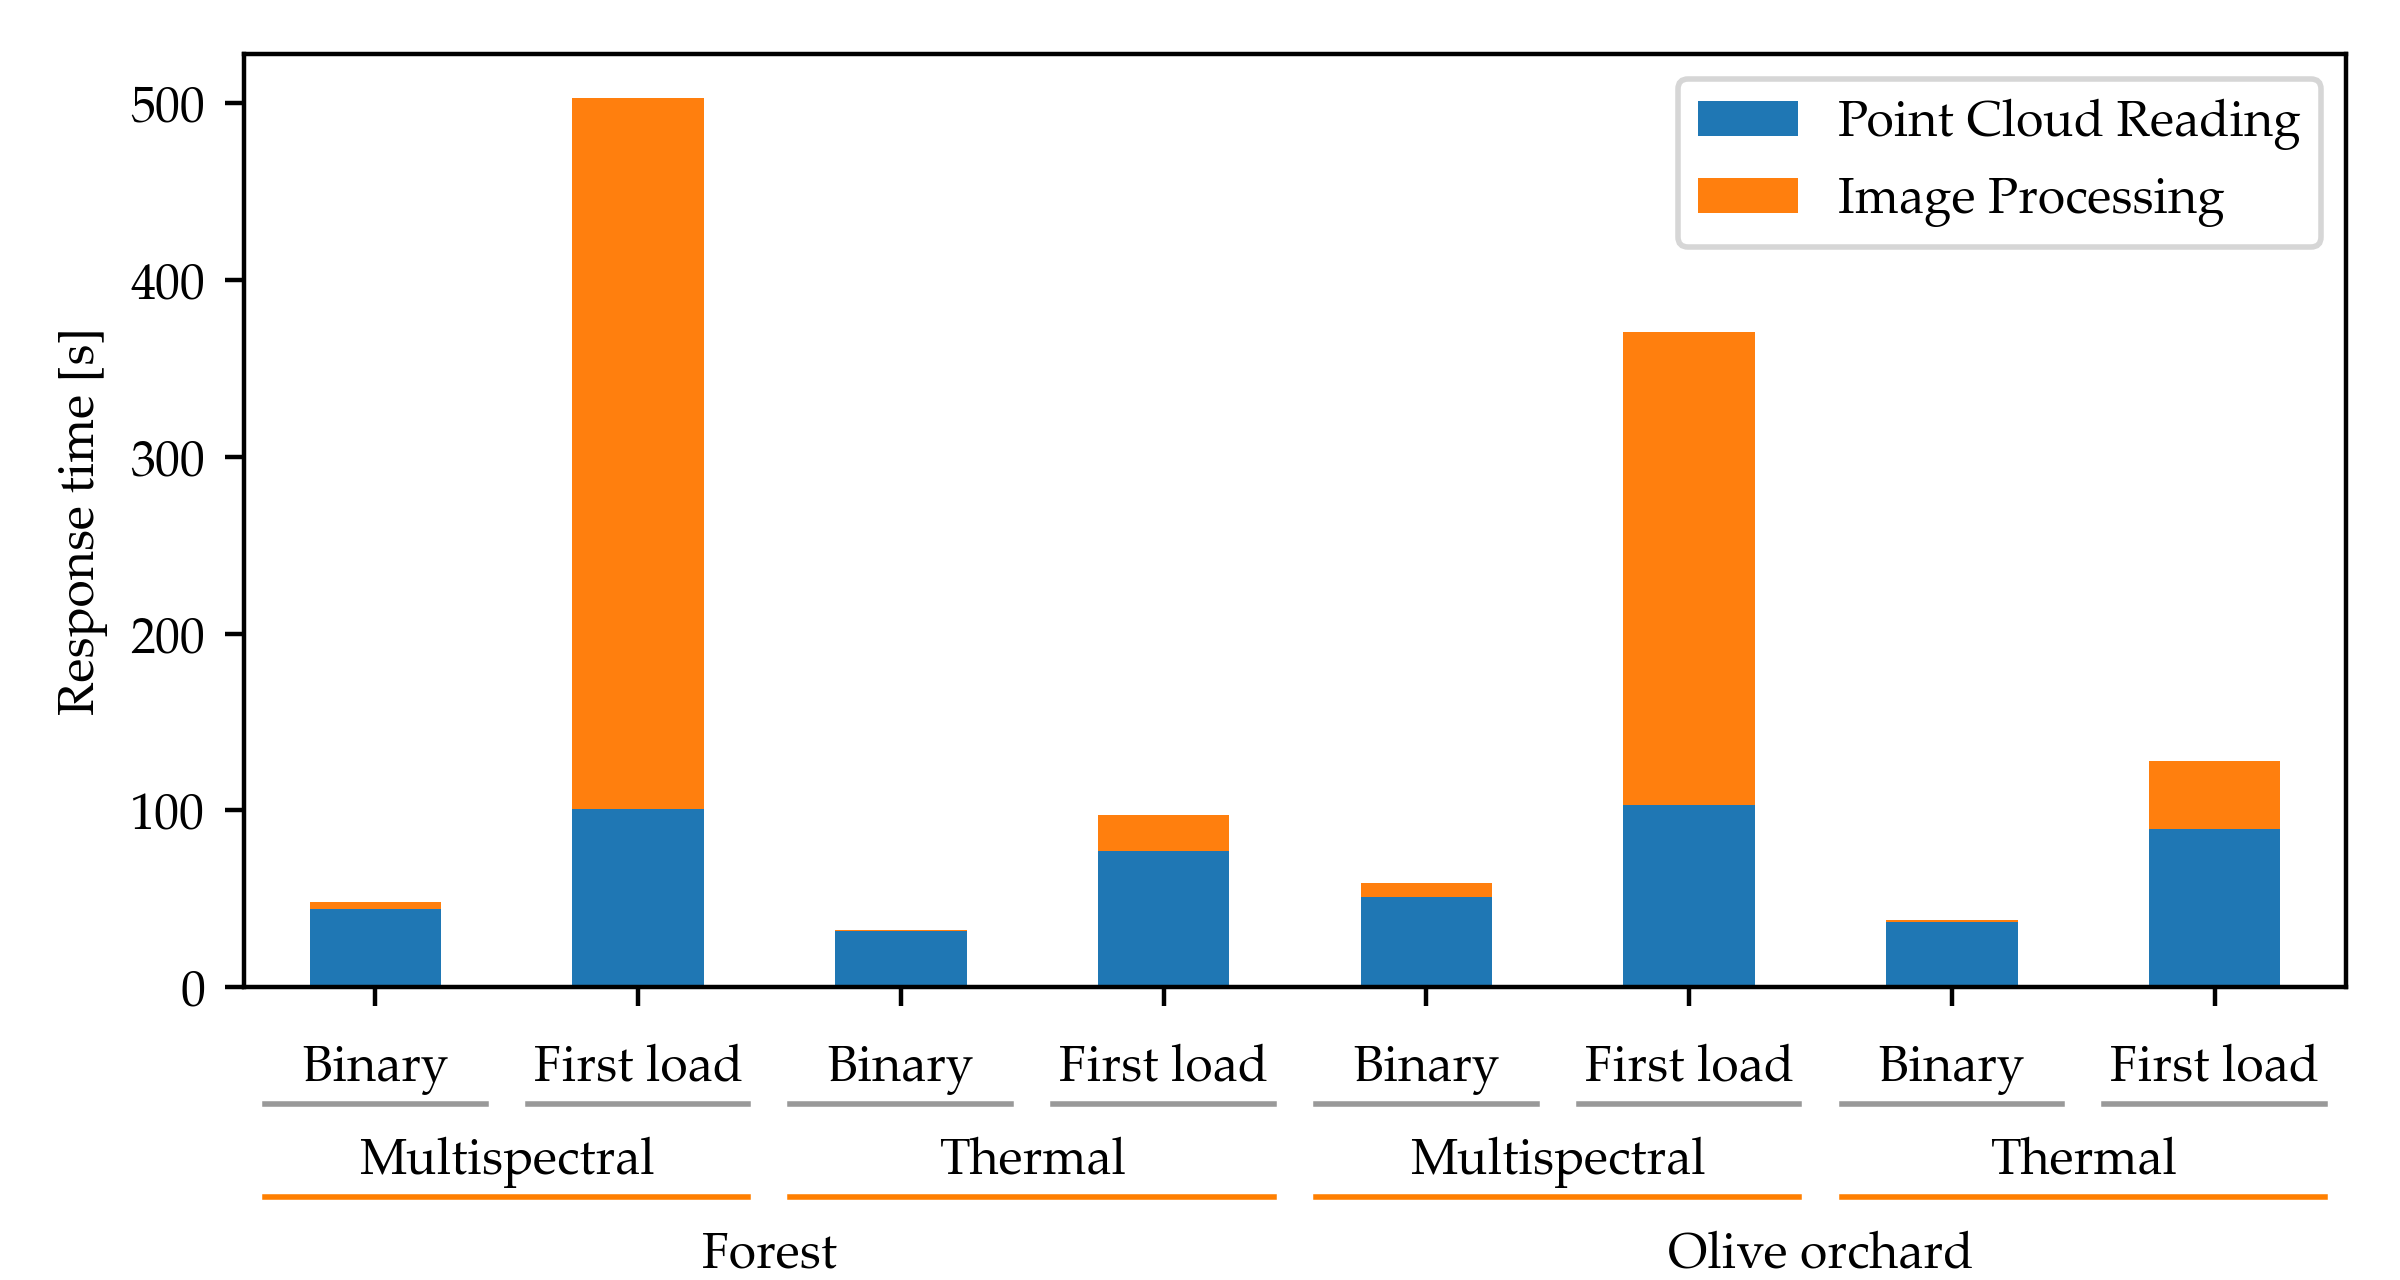
\includegraphics[width=\linewidth]{figs/multi_thermal_projection/results/binary_response_time.png}
    \hspace*{\fill}
    \caption{Comparison of latency for the first two stages of our method in the first and subsequent loads (after storing calculated data in binary files).}
	\label{fig:occlusion_binary_response_time}
\end{figure}

\renewcommand{\arraystretch}{1.2}
\begin{table}
    \centering
    \caption{Response time of the first two stages if 1) it is the first load or 2) binary data has already been stored as a result of a previous load. \textbf{Stage 1} refers to point cloud reading, whereas \textbf{Stage 2} involves the image processing prior to the dense reconstruction.  }
    \label{table:binary_results}
    \begin{tabular}{l|rr|rr}
    \toprule
    & \multicolumn{2}{c}{Binary} & \multicolumn{2}{c}{First load}\\
    \cmidrule{1-5}
    \textbf{Dataset} & \textbf{Stage 1} & \textbf{Stage 2} & \textbf{Stage 1} & \textbf{Stage 2}\\
    \cmidrule{1-5}
    a) Therm., i) Forest & \textbf{0.61 \si{\minute}} & \textbf{0.01 \si{\minute}} & 1.48 \si{\minute} & 0.64 \si{\minute}\\
    \cmidrule{1-5}
    a) Therm., ii) Olive orch. & \textbf{0.52 \si{\minute}} & \textbf{0.01 \si{\minute}} & 1.28 \si{\minute} & 0.34 \si{\minute}\\
    \cmidrule{1-5}
    b) Mult., i) Forest & \textbf{0.85 \si{\minute}} & \textbf{0.12 \si{\minute}} & 1.71 \si{\minute} & 4.45 \si{\minute}\\
    \cmidrule{1-5}
    b) Mult., ii) Olive orch. & \textbf{0.73 \si{\minute}} & \textbf{0.06 \si{\minute}} & 1.67 \si{\minute} & 6.69 \si{\minute}\\
    \bottomrule
    \end{tabular}
\end{table}
\renewcommand{\arraystretch}{1}

\section{Conclusions and future work}

The reconstruction of multiple 3D point clouds is a common task in surveying work. Although it may solely include visible imagery, it is frequent to include other sensors that shed light on some of the features of the studied field. For instance, archaeological work in Remote Sensing can be supported by thermographic imaging. Hence, the reconstruction of 3D point clouds of further data sources, such as thermal and multispectral, can be performed by taking advantage of previous RGB reconstructions. Although all of them can be performed with commercial software, we identified several drawbacks, including 1) high response time, 2) low point density and 3) incorrect estimations without further knowledge, e.g., GCPs. The latter drawback occurs due to the lower dimensionality and higher number of defects of thermal and multispectral imagery, thus hardening the recognition of image features.

We proposed to integrate the reconstruction of thermal and multispectral 3D point clouds in an accelerated projection-based methodology. To this end, the reconstruction of RGB point clouds was performed with traditional software. Then, the subsequent reconstructions were done with much less latency (approximately -77\%) and yielded point clouds whose size increase was above 140\%. Accordingly, the latency results were improved whether they were normalized according to the point cloud's size (> 95\%). Despite both commercial software and our method using GPU-accelerated procedures, ours was shown to outperform two widespread solutions in terms of response time and size. 

Still, GPU parallelism was implemented with GLSL, which provides little flexibility and control of the execution pipeline (e.g., overlapping data transfers and thread logic). Furthermore, it runs over a single GPU as it is part of a rendering framework. As a future work, the GPGPU solution could transit to a flexible and multi-GPU framework such as CUDA. Although its results were worse for a single GPU, it can greatly benefit from a multi-GPU configuration to outperform OpenGL-based approaches. Regarding the explored data, further data sources could be integrated into the multi-layer point cloud, such as hyperspectral reflectance. Finally, instead of performing the projection over RGB point clouds, LiDAR outcome could be used as a dense point cloud where other data sources are projected.  

\begin{table*}[hb]
    \centering
    \caption{Graphic results of the dense reconstruction of 1) Agisoft Metashape, 2) Pix4Dmapper and 3) our proposed method. Multispectral point clouds are rendered according to the GRE band. }
    \label{table:visual_results}  
    \newcommand\imageTableSize{0.32\textwidth}
    \begin{tabular}{l|c|c|c}
    \toprule
    \textbf{Configuration} & \textbf{Data source} &\textbf{Dataset 1} & \textbf{Dataset 2}\\
    \cmidrule{1-4}
    \multirow{2}{*}[-4em]{A. Metashape} & Thermal & \multicolumn{1}{m{\imageTableSize}|}{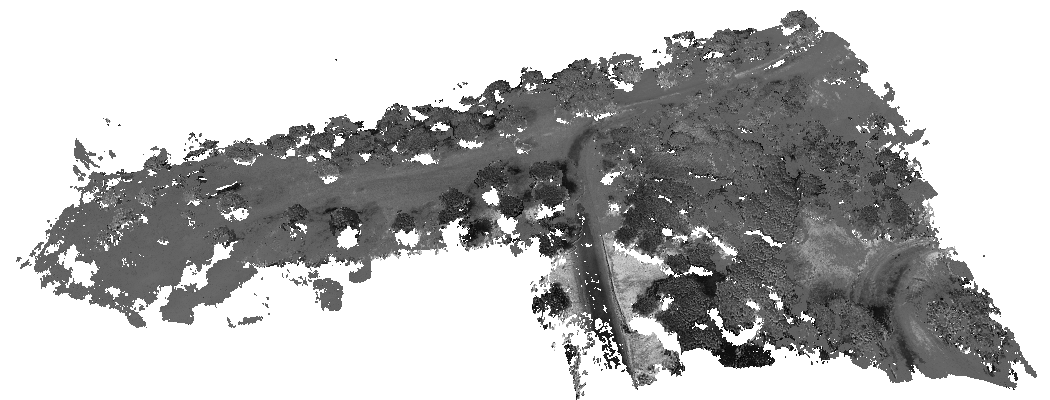
\includegraphics[width=\imageTableSize]{figs/multi_thermal_projection/results/metashape/AgisoftThermalMarmolejo.png}} & \multicolumn{1}{m{\imageTableSize}}{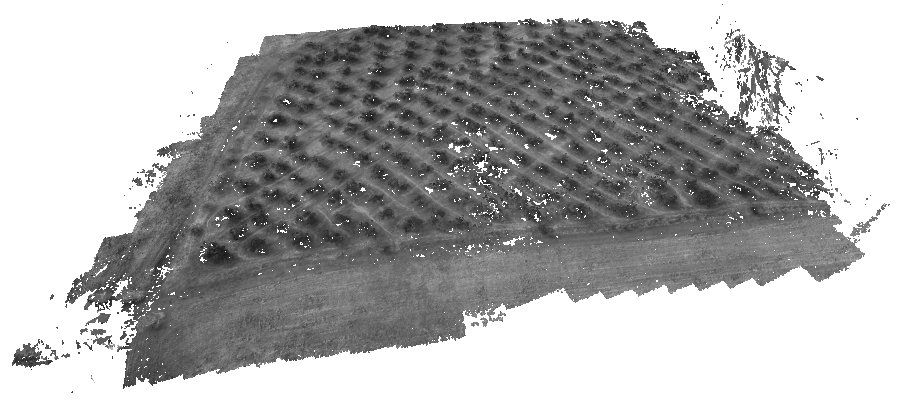
\includegraphics[width=\imageTableSize]{figs/multi_thermal_projection/results/metashape/AgisoftThermalNovember.png}}\\
    & Multispectral & \multicolumn{1}{m{\imageTableSize}|}{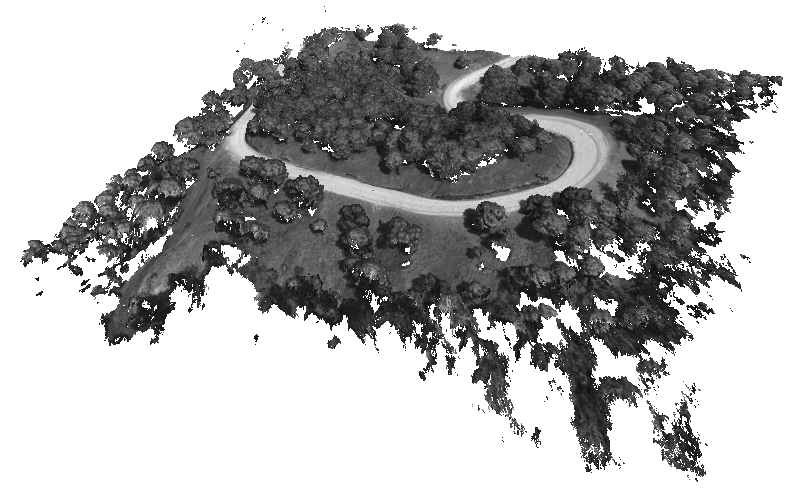
\includegraphics[width=\imageTableSize]{figs/multi_thermal_projection/results/metashape/AgisoftMultispectralMarmolejo.png}} & \multicolumn{1}{m{\imageTableSize}}{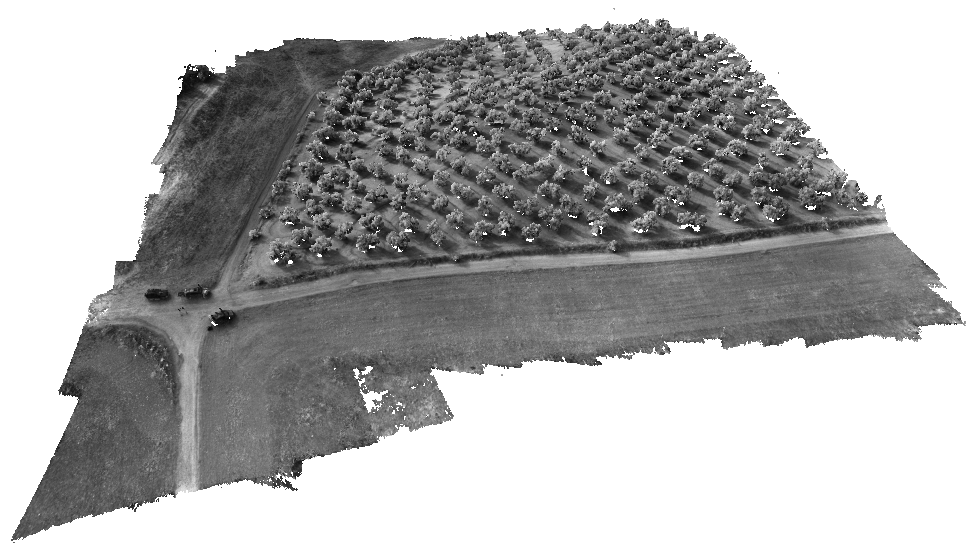
\includegraphics[width=\imageTableSize]{figs/multi_thermal_projection/results/metashape/AgisoftMultispectralNovember.png}}\\
    \cmidrule{1-4}
    \multirow{2}{*}[-4.3em]{Pix4Dmapper} & Thermal & \multicolumn{1}{m{\imageTableSize}|}{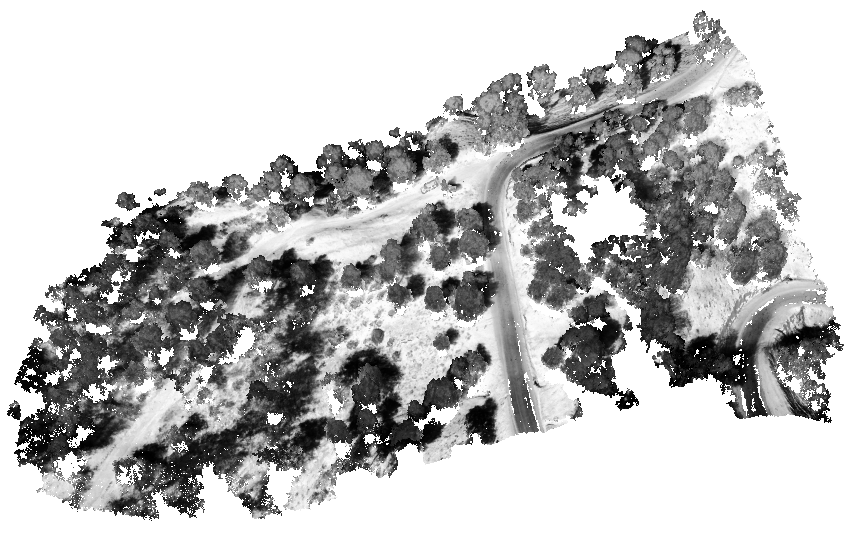
\includegraphics[width=\imageTableSize]{figs/multi_thermal_projection/results/pix4dmapper/Pix4DThermalMarmolejo.png}} & \multicolumn{1}{m{\imageTableSize}}{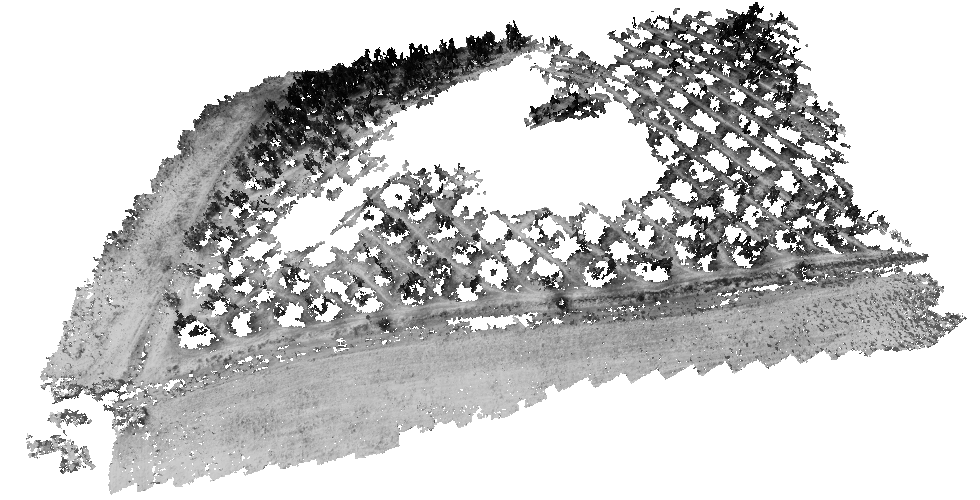
\includegraphics[width=\imageTableSize]{figs/multi_thermal_projection/results/pix4dmapper/Pix4DThermalNovember.png}}\\
    & Multispectral & \multicolumn{1}{m{\imageTableSize}|}{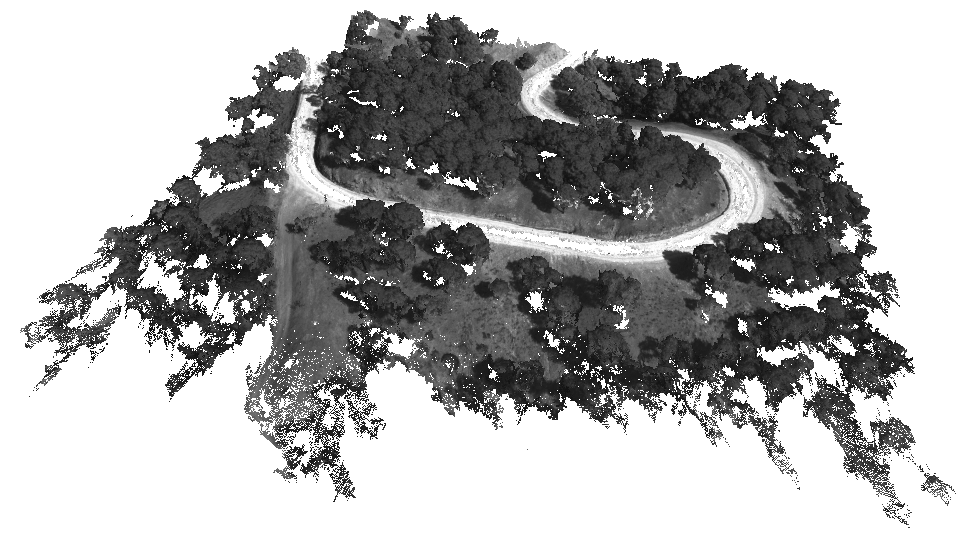
\includegraphics[width=\imageTableSize]{figs/multi_thermal_projection/results/pix4dmapper/Pix4DMultispectralMarmolejo.png}} & \multicolumn{1}{m{\imageTableSize}}{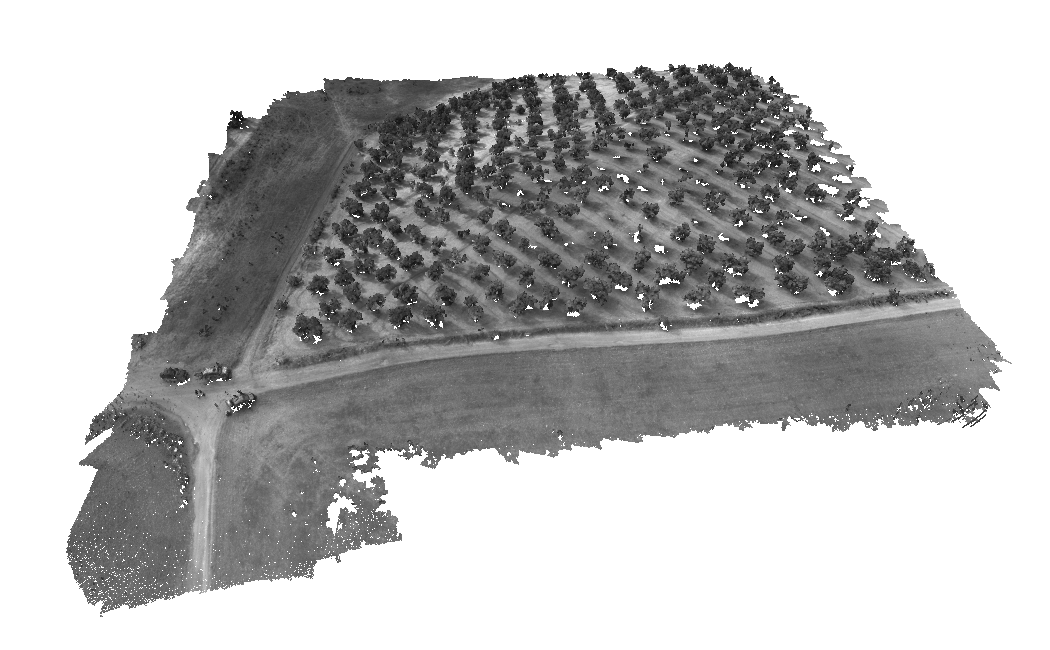
\includegraphics[width=\imageTableSize]{figs/multi_thermal_projection/results/pix4dmapper/Pix4DMultispectralNovember.png}}\\
    \cmidrule{1-4}
    \multirow{2}{*}[-4.3em]{Our method} & Thermal & \multicolumn{1}{m{\imageTableSize}|}{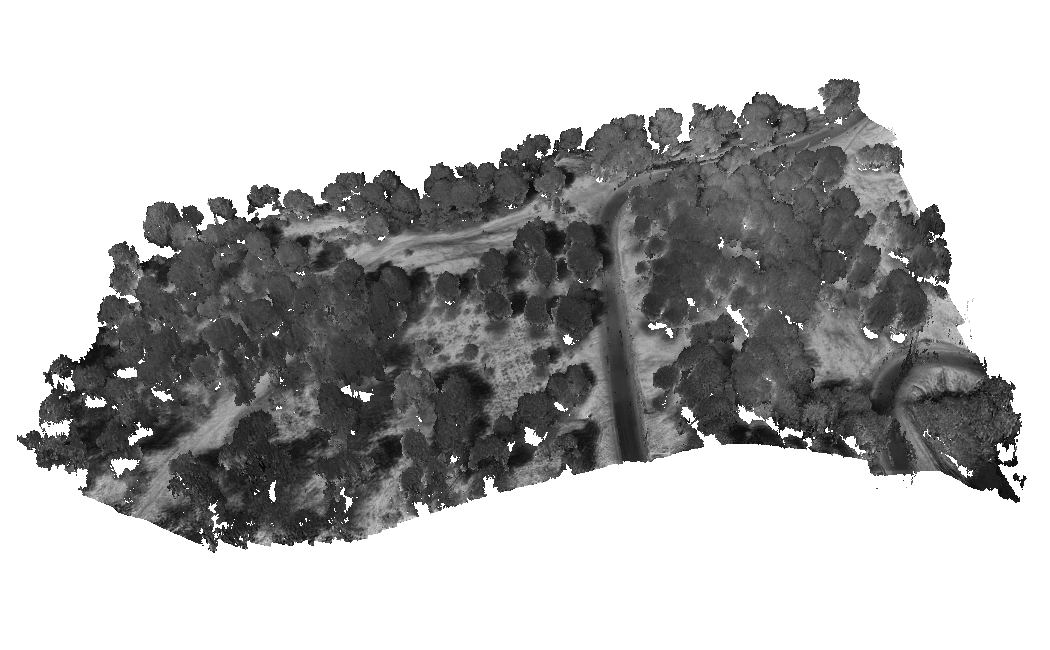
\includegraphics[width=\imageTableSize]{figs/multi_thermal_projection/results/ours/OurThermalMarmolejo.png}} & \multicolumn{1}{m{\imageTableSize}}{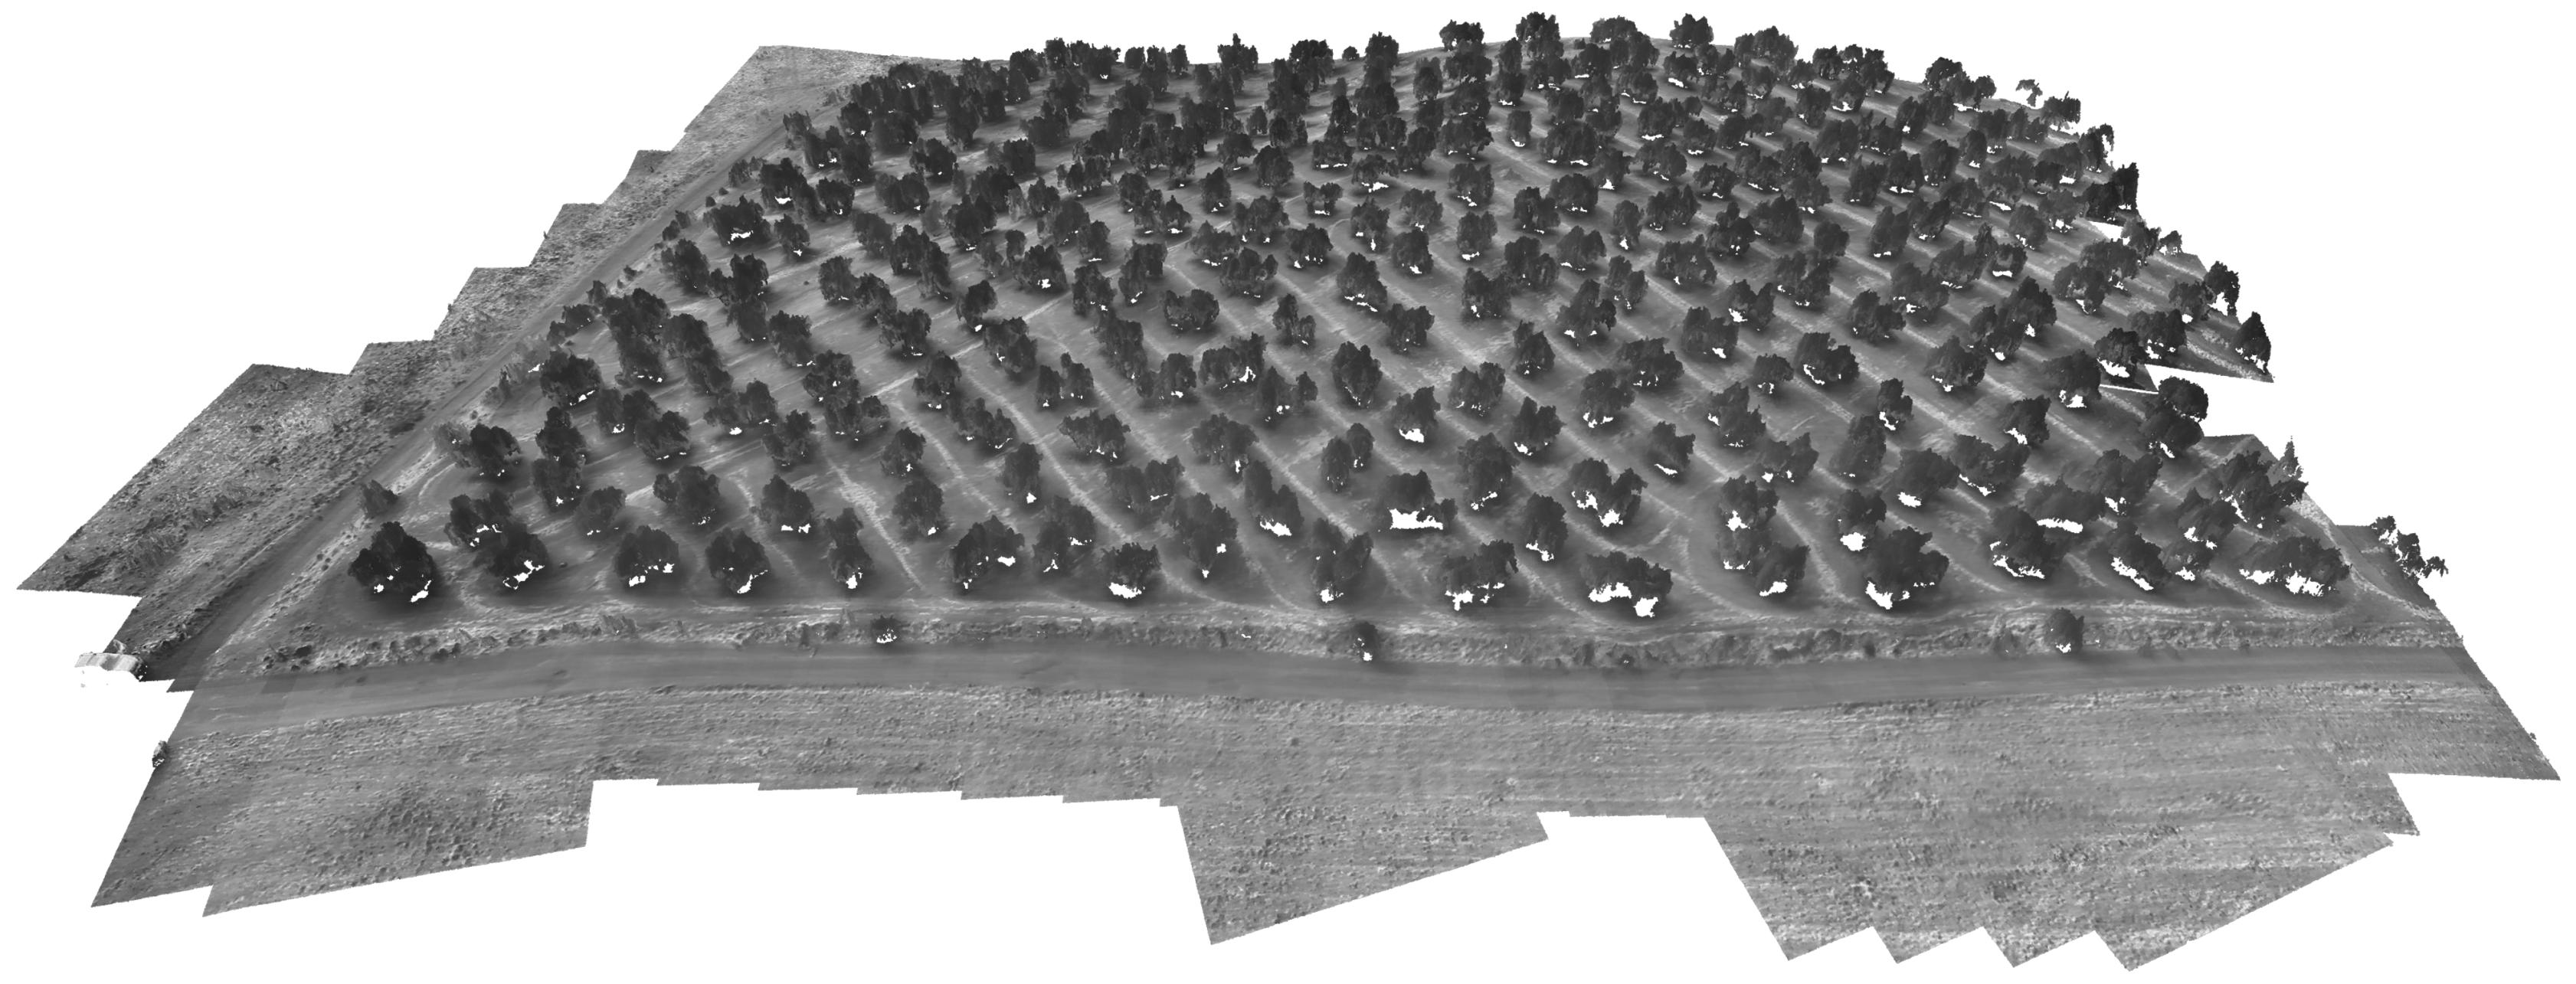
\includegraphics[width=\imageTableSize]{figs/multi_thermal_projection/results/ours/OurThermalNovember2.png}}\\
    & Multispectral & \multicolumn{1}{m{\imageTableSize}|}{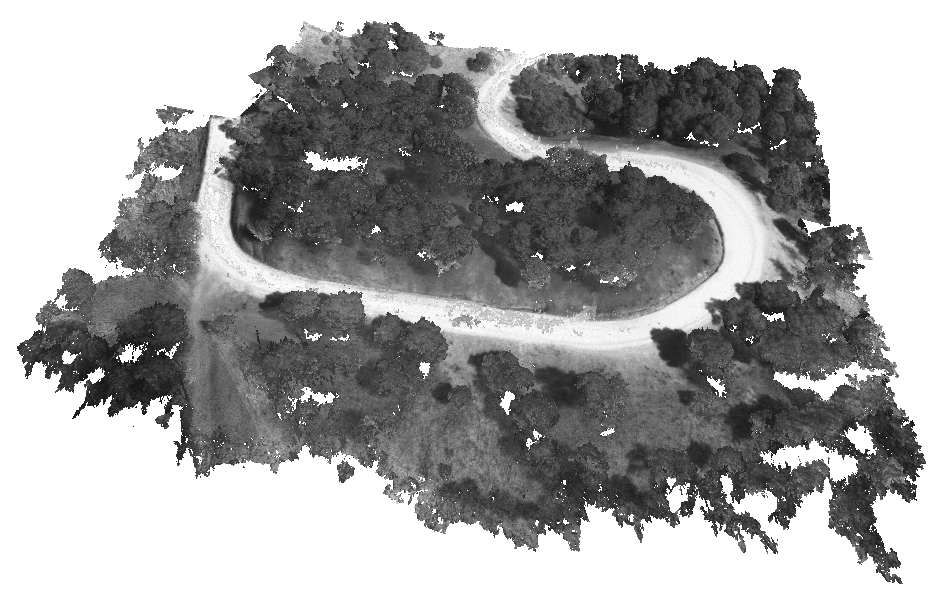
\includegraphics[width=\imageTableSize]{figs/multi_thermal_projection/results/ours/OurMultispectralMarmolejo.png}} & \multicolumn{1}{m{\imageTableSize}}{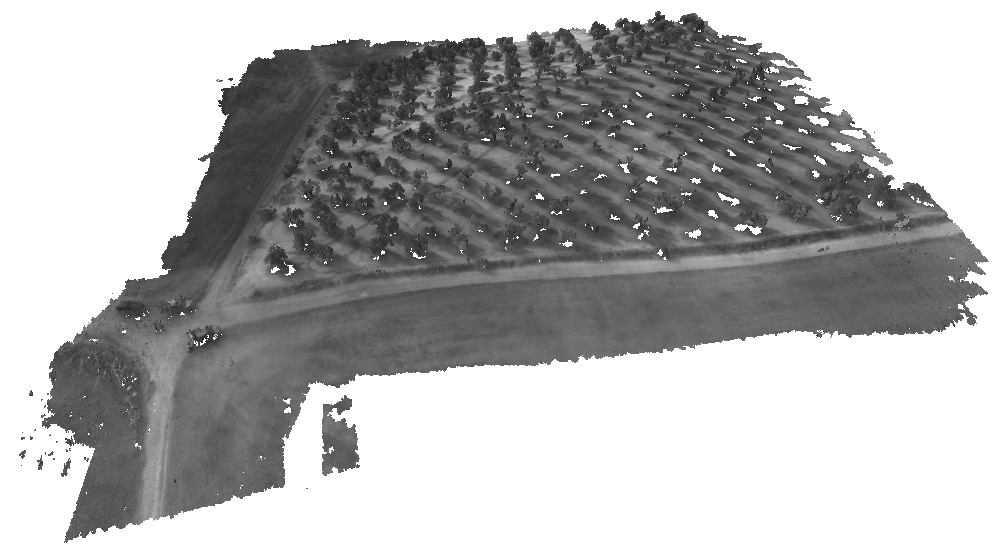
\includegraphics[width=\imageTableSize]{figs/multi_thermal_projection/results/ours/OurMultispectralNovember.png}}\\
    \bottomrule
    \end{tabular}
\end{table*}

